\documentclass[a4paper, oneside, dvipsnames, table]{article}
\usepackage{../../Utilita/Stiletemplate}
\usepackage{hyperref}
\usepackage{fancyhdr}
\usepackage{amsfonts}
\usepackage{amsmath}
\usepackage[italian]{babel}
\setcounter{tocdepth}{5}
\setcounter{secnumdepth}{5}

\newcommand{\Titolo}{Piano di Qualifica}

\newcommand{\Redattori}{\AT{} \newline \MC{} \newline \BR{}}

\newcommand{\Verificatori}{\LD{} \newline \DF{}}

\newcommand{\Approvatore}{\SE{}}

\newcommand{\Distribuzione}{\Proponente{} \newline \VT{} \newline \CR{} \newline Gruppo \Gruppo{}}

\newcommand{\Uso}{Esterno}

\newcommand{\DescrizioneDoc}{Questo documento si occupa di descrivere il \PdQ{} realizzato dal Gruppo \Gruppo{} per il progetto \NomeProgetto{}.}

\newcommand{\pathimg}{../../Utilita/Immagini/qbteam.png}

\newcommand{\Versionedoc}{2.0.0}
% scritto da \DF{},\AT{}

% info generali 
\newcommand{\NomeProgetto}{\textit{Stalker}}

% fornitore
\newcommand{\Gruppo}{\textit{qbteam}}
\newcommand{\Mail}{qbteamswe@gmail.com}
% \newcommand{\pathimg}{Immagini/qbteam.png}

% committenti
\newcommand{\Committente}{\VT \newline \CR}
\newcommand{\VT}{Prof. Vardanega Tullio}
\newcommand{\CR}{Prof. Cardin Riccardo}

% proponenti
\newcommand{\Proponente}{\textit{Imola Informatica}}
\newcommand{\ZD}{Zanetti Davide}
\newcommand{\CT}{Cardona Tommaso}

% qbteam
\newcommand{\AT}{Azzalin Tommaso}
\newcommand{\DF}{Drago Francesco}
\newcommand{\BR}{Baratin Riccardo}
\newcommand{\MC}{Mattei Christian}
\newcommand{\PF}{Perin Federico}
\newcommand{\CE}{Cisotto Emanuele}
\newcommand{\SE}{Salmaso Enrico}
\newcommand{\LD}{Lazzaro Davide}

% ruoli
\newcommand{\Responsabile}{Responsabile di Progetto}
\newcommand{\Amministratore}{Amministratore di Progetto}

% documenti

\newcommand{\SdF}{Studio di Fattibilità}
\newcommand{\SdFv}[1]{\textit{Studio di Fattibilità {#1}}}
\newcommand{\PdQ}{Piano di Qualifica}
\newcommand{\PdQv}[1]{\textit{Piano di Qualifica {#1}}}
\newcommand{\PdP}{Piano di Progetto}
\newcommand{\PdPv}[1]{\textit{Piano di Progetto {#1}}}
\newcommand{\NdP}{Norme di Progetto}
\newcommand{\NdPv}[1]{\textit{Norme di Progetto {#1}}}
\newcommand{\AdR}{Analisi dei Requisiti}
\newcommand{\AdRv}[1]{\textit{Analisi dei Requisiti {#1}}}
\newcommand{\Glossario}{Glossario}
\newcommand{\Glossariov}[1]{\textit{Glossario {#1}}}
\newcommand{\MM}{Manuale Manutentore}
\newcommand{\MU}{Manuale Utente}

% comandi generali
\newcommand{\glo}[1]{#1\ap{G}}

\setlength{\parindent}{-0.1em}


\begin{document}

\copertina{}
\newpage

\section*{Registro delle modifiche}
{
\rowcolors{2}{grigetto}{white}
\renewcommand{\arraystretch}{1.5}
\centering
\begin{longtable}{ c c  C{2.3cm} c C{3cm} C{3.2cm}}
\rowcolor{rossoep}
\textcolor{white}{\textbf{Versione}} & \textcolor{white}{\textbf{Data}} & \textcolor{white}{\textbf{Nominativo}} & \textcolor{white}{\textbf{Ruolo}} & 
\textcolor{white}{\textbf{Verificatore}}& \textcolor{white}{\textbf{Descrizione}}\\	


1.0.0 & \Data & \CE{} & Responsabili & \CE{} & Approvazione per il rilascio.  \\
		
0.0.1 & \Data & \DF{} & Analista & \AT{} & Stesura e verifica del documento.  \\
		
		
\end{longtable}
}


\fancydoc{}

\clearpage
\tableofcontents
\clearpage

% scritto da\AT{}
\section{Introduzione}
\subsection{Scopo del documento}
Il presente documento ha lo scopo di descrivere le strategie che il gruppo \Gruppo{} intende applicare per garantire la qualità di processo e di prodotto per l’intera durata del progetto.
Al fine di rispettare questi obiettivi vengono descritte le modalità in cui vengono effettuate la verifica e la validazione del prodotto.
In questo modo è consentita la rilevazione e correzione di problemi o incongruenze in breve tempo, senza correre il rischio di sprechi di risorse.

\subsection{Scopo generale del prodotto}
L'obiettivo del prodotto \NomeProgetto{} di \Proponente{} è la creazione di un sistema software composto di un applicativo per cellulare e di un server, con cui interagire tramite un'interfaccia utente. La necessità nasce dal bisogno di adempiere alle normative vigenti in tema di sicurezza.
Le due componenti del sistema software, applicativo e server, devono soddisfare i seguenti obiettivi rispettivamente di:
\begin{itemize}
\item Tracciare e registrare i \glo{movimenti} di un utente in un \glo{luogo di tracciamento} di un'\glo{organizzazione}, siano essi autenticati da credenziali di un'\glo{organizzazione} oppure visitatori anonimi, il tutto nel rispetto della normativa sulla privacy;
\item Poter visionare gli accessi degli utenti autenticati e visionare il numero di visitatori anonimi all'interno di un luogo.
\end{itemize}

\subsection{Glossario}
Al fine di evitare ambiguità fra i termini, e per avere chiare fra tutti gli stakeholder le terminologie utilizzate per la realizzazione del presente documento, il gruppo \Gruppo{} ha redatto un documento denominato \Glossariov{1.0.0}.
In tale documento, sono presenti tutti i termini tecnici, ambigui, specifici del progetto e scelti dai membri del gruppo con le loro relative definizioni.
Un termine presente nel \Glossariov{1.0.0} e utilizzato in questo documento viene indicato con un apice \ap{G} alla fine della parola.

\subsection{Standard di progetto}
Il gruppo \Gruppo{} ha deciso di gestire i propri processi del ciclo di vita del software adottando alcune parti dello standard \textbf{ISO/IEC 12207} come definito nelle \textit{NormeDiProgetto}; 
come modello di qualità del prodotto software si è utilizzato parte dello standard \textbf{ISO/IEC 9126} anch'esso definito nelle \textit{NormeDiProgetto}.

\subsection{Riferimenti}

\subsubsection{Normativi}
\begin{itemize}
    \item \textbf{Capitolato d'appalto C5 - Stalker}\\     
    \url{https://www.math.unipd.it/~tullio/IS-1/2019/Progetto/C5.pdf};
    \item \NdPv{1.0.0}.
    \item \textbf{ISO/IEC 12207-1995:}\\     
    \url{https://www.math.unipd.it/~tullio/IS-1/2009/Approfondimenti/ISO_12207-1995.pdf};\\
    \url{http://www.colonese.it/SviluppoSw_Standard_ISO12207.html};
    \item \textbf{ISO/IEC 9126:}\\
    \url{http://www.colonese.it/00-Manuali_Pubblicatii/07-ISO-IEC9126_v2.pdf};\\
    \url{https://en.wikipedia.org/wiki/ISO/IEC_9126};
\end{itemize}

\subsubsection{Informativi}
\begin{itemize}
    \item \textbf{Indice di Gulpease}\\
    \url{https://it.wikipedia.org/wiki/Indice_Gulpease};
    \item \textbf{Metriche di progetto}\\
    \url{https://it.wikipedia.org/wiki/Metriche_di_progetto};
    \item \textbf{Varie metriche}\\
    \url{http://torlone.dia.uniroma3.it/sistelab/annipassati/sbavaglia.pdf};
    \item \textbf{Ciclo di Deming - Plan Do Check Act}\\
    \url{https://it.wikipedia.org/wiki/Ciclo_di_Deming};
    
\end{itemize}
\clearpage

\section{Processi primari}
\subsection{Processo di fornitura}
\subsubsection{Scopo}
Lo scopo della seguente sezione è formalizzare le norme e le procedure che il gruppo \Gruppo{} deve applicare al fine di diventare fornitore del proponente \Proponente{} e dei committenti \VT{} e \CR{}.

\subsubsection{Prospettiva}
Il gruppo si impegnerà a mantenere un rapporto costante con il proponente per poter riuscire ad applicare le seguenti procedure:
\begin{itemize}
	\item comprendere e redigere i requisiti richiesti dal proponente;
	\item chiarire qualsiasi domanda del proponente;
	\item fornire eventuali spiegazioni del costo per la realizzazione del progetto \NomeProgetto{};
	\item approssimare le tempistiche di lavoro per tenere aggiornato continuamente il proponente sullo stato del prodotto; 
	\item far capire al proponente ciò che è possibile implementare;
\end{itemize}

\subsubsection{Descrizione} 
Il processo primario di fornitura ha l'obiettivo di capire e comprendere tutte le richieste del proponente, redigendo uno studio di fattibilità. 
Il gruppo \Gruppo{} ha il compito di valutare tali richieste e tenere in considerazione le risorse necessarie ai fini del progetto, esponendo al proponente \Proponente{} le attività che intende svolgere per realizzare il prodotto richiesto.
Tutte queste informazioni vengono inserite nel \PdP{}, il quale deve accompagnare il gruppo per tutta la durata del progetto.
Il gruppo \Gruppo{} deve cercare di essere il più possibile in contatto con il proponente per poter comprendere i suoi bisogni.\\

\input{Sezioni/Sottosezioni/Attività.tex}

%inizio parte scritta da \PF{}
\subsection{Processo di sviluppo}
\subsubsection{Scopo}
Lo scopo del processo di sviluppo è quello di contenere compiti e attività da svolgere, in modo tale da poter fornire al proponente il prodotto finale da lui richiesto.\\
Per una corretta implementazione del prodotto software devono essere svolti i seguenti punti: 
\begin{itemize}
	\item Fissare gli obiettivi di sviluppo;
	\item Fissare i vincoli tecnologici e di design;
	\item Realizzare un prodotto finale che soddisfi tutti i test di \glo{verifica} e \glo{validazione} i quali devono rispettare quanto definito dal piano di qualità;
	\item Realizzare un prodotto finale conforme ai \glo{requisiti} richiesti dal proponente.
\end{itemize}
\subsubsection{Descrizione}
Il processo di sviluppo è formato da attività e compiti che fanno parte del ciclo di vita del prodotto software, il quale deve soddisfare tutti i \glo{requisiti} indicati nelle specifiche dal proponente per poter essere accettato.		
Il \glo{processo} di sviluppo come detto in precedenza è formato dalle seguenti attività:
\begin{itemize}
	\item \textbf{Analisi dei Requisiti}: Attività in cui si cerca di capire appieno il problema presentato dal cliente ricavando i \glo{requisiti} da soddisfare nella realizzazione del prodotto;
	\item \textbf{Progettazione}: Attività che segue l'analisi dei requisiti nella quale si stabilisce come devono essere realizzati i \glo{requisiti} imposti cliente;
	\item \textbf{Codifica}: Attività in cui si realizza concretamente quello che nel progetto è stato  studiato precedentemente;
	\item \textbf{Test}: Attività in cui si verifica che ogni pezzo di codice scritto durante l'attività di codifica sia privo di errori. Il tutto deve risultare conforme alle aspettative prefissate precedentemente nella way of working;
	\item \textbf{Collaudo}: Attività svolta in concomitanza con il proponente in cui si esegue un test finale che dimostri che il prodotto software realizzato soddisfa tutti i \glo{requisiti} presenti nel capitolato.
\end{itemize}
%fine parte scritta da \PF{}

\documentclass[a4paper, oneside, dvipsnames, table]{article}
\usepackage{../../Utilita/Stiletemplate}
\usepackage{hyperref}
\usepackage{fancyhdr}
\usepackage[italian]{babel}
\usepackage[raggedright]{titlesec}
\usepackage{blindtext}
\usepackage[export]{adjustbox}
\titleformat{\paragraph}[hang]{\normalfont\normalsize\bfseries}{\theparagraph}{1em}{}
\titlespacing*{\paragraph}{0pt}{3.25ex plus 1ex minus .2ex}{0.5em}

\newcommand{\Titolo}{Piano di Qualifica}

\newcommand{\Redattori}{\AT{} \newline \MC{} \newline \BR{}}

\newcommand{\Verificatori}{\LD{} \newline \DF{}}

\newcommand{\Approvatore}{\SE{}}

\newcommand{\Distribuzione}{\Proponente{} \newline \VT{} \newline \CR{} \newline Gruppo \Gruppo{}}

\newcommand{\Uso}{Esterno}

\newcommand{\DescrizioneDoc}{Questo documento si occupa di descrivere il \PdQ{} realizzato dal Gruppo \Gruppo{} per il progetto \NomeProgetto{}.}

\newcommand{\pathimg}{../../Utilita/Immagini/qbteam.png}

\newcommand{\Versionedoc}{2.0.0}
% scritto da \DF{},\AT{}

% info generali 
\newcommand{\NomeProgetto}{\textit{Stalker}}

% fornitore
\newcommand{\Gruppo}{\textit{qbteam}}
\newcommand{\Mail}{qbteamswe@gmail.com}
% \newcommand{\pathimg}{Immagini/qbteam.png}

% committenti
\newcommand{\Committente}{\VT \newline \CR}
\newcommand{\VT}{Prof. Vardanega Tullio}
\newcommand{\CR}{Prof. Cardin Riccardo}

% proponenti
\newcommand{\Proponente}{\textit{Imola Informatica}}
\newcommand{\ZD}{Zanetti Davide}
\newcommand{\CT}{Cardona Tommaso}

% qbteam
\newcommand{\AT}{Azzalin Tommaso}
\newcommand{\DF}{Drago Francesco}
\newcommand{\BR}{Baratin Riccardo}
\newcommand{\MC}{Mattei Christian}
\newcommand{\PF}{Perin Federico}
\newcommand{\CE}{Cisotto Emanuele}
\newcommand{\SE}{Salmaso Enrico}
\newcommand{\LD}{Lazzaro Davide}

% ruoli
\newcommand{\Responsabile}{Responsabile di Progetto}
\newcommand{\Amministratore}{Amministratore di Progetto}

% documenti

\newcommand{\SdF}{Studio di Fattibilità}
\newcommand{\SdFv}[1]{\textit{Studio di Fattibilità {#1}}}
\newcommand{\PdQ}{Piano di Qualifica}
\newcommand{\PdQv}[1]{\textit{Piano di Qualifica {#1}}}
\newcommand{\PdP}{Piano di Progetto}
\newcommand{\PdPv}[1]{\textit{Piano di Progetto {#1}}}
\newcommand{\NdP}{Norme di Progetto}
\newcommand{\NdPv}[1]{\textit{Norme di Progetto {#1}}}
\newcommand{\AdR}{Analisi dei Requisiti}
\newcommand{\AdRv}[1]{\textit{Analisi dei Requisiti {#1}}}
\newcommand{\Glossario}{Glossario}
\newcommand{\Glossariov}[1]{\textit{Glossario {#1}}}
\newcommand{\MM}{Manuale Manutentore}
\newcommand{\MU}{Manuale Utente}

% comandi generali
\newcommand{\glo}[1]{#1\ap{G}}

\setlength{\parindent}{-0.1em}


\begin{document}

\copertina{}
\newpage

\section*{Registro delle modifiche}
{
\rowcolors{2}{grigetto}{white}
\renewcommand{\arraystretch}{1.5}
\centering
\begin{longtable}{ c c  C{2.3cm} c C{3cm} C{3.2cm}}
\rowcolor{rossoep}
\textcolor{white}{\textbf{Versione}} & \textcolor{white}{\textbf{Data}} & \textcolor{white}{\textbf{Nominativo}} & \textcolor{white}{\textbf{Ruolo}} & 
\textcolor{white}{\textbf{Verificatore}}& \textcolor{white}{\textbf{Descrizione}}\\	


1.0.0 & \Data & \CE{} & Responsabili & \CE{} & Approvazione per il rilascio.  \\
		
0.0.1 & \Data & \DF{} & Analista & \AT{} & Stesura e verifica del documento.  \\
		
		
\end{longtable}
}

\fancydoc{}

\clearpage
\tableofcontents
\clearpage
\listoffigures
\clearpage

% scritto da\AT{}
\section{Introduzione}
\subsection{Scopo del documento}
Il presente documento ha lo scopo di descrivere le strategie che il gruppo \Gruppo{} intende applicare per garantire la qualità di processo e di prodotto per l’intera durata del progetto.
Al fine di rispettare questi obiettivi vengono descritte le modalità in cui vengono effettuate la verifica e la validazione del prodotto.
In questo modo è consentita la rilevazione e correzione di problemi o incongruenze in breve tempo, senza correre il rischio di sprechi di risorse.

\subsection{Scopo generale del prodotto}
L'obiettivo del prodotto \NomeProgetto{} di \Proponente{} è la creazione di un sistema software composto di un applicativo per cellulare e di un server, con cui interagire tramite un'interfaccia utente. La necessità nasce dal bisogno di adempiere alle normative vigenti in tema di sicurezza.
Le due componenti del sistema software, applicativo e server, devono soddisfare i seguenti obiettivi rispettivamente di:
\begin{itemize}
\item Tracciare e registrare i \glo{movimenti} di un utente in un \glo{luogo di tracciamento} di un'\glo{organizzazione}, siano essi autenticati da credenziali di un'\glo{organizzazione} oppure visitatori anonimi, il tutto nel rispetto della normativa sulla privacy;
\item Poter visionare gli accessi degli utenti autenticati e visionare il numero di visitatori anonimi all'interno di un luogo.
\end{itemize}

\subsection{Glossario}
Al fine di evitare ambiguità fra i termini, e per avere chiare fra tutti gli stakeholder le terminologie utilizzate per la realizzazione del presente documento, il gruppo \Gruppo{} ha redatto un documento denominato \Glossariov{1.0.0}.
In tale documento, sono presenti tutti i termini tecnici, ambigui, specifici del progetto e scelti dai membri del gruppo con le loro relative definizioni.
Un termine presente nel \Glossariov{1.0.0} e utilizzato in questo documento viene indicato con un apice \ap{G} alla fine della parola.

\subsection{Standard di progetto}
Il gruppo \Gruppo{} ha deciso di gestire i propri processi del ciclo di vita del software adottando alcune parti dello standard \textbf{ISO/IEC 12207} come definito nelle \textit{NormeDiProgetto}; 
come modello di qualità del prodotto software si è utilizzato parte dello standard \textbf{ISO/IEC 9126} anch'esso definito nelle \textit{NormeDiProgetto}.

\subsection{Riferimenti}

\subsubsection{Normativi}
\begin{itemize}
    \item \textbf{Capitolato d'appalto C5 - Stalker}\\     
    \url{https://www.math.unipd.it/~tullio/IS-1/2019/Progetto/C5.pdf};
    \item \NdPv{1.0.0}.
    \item \textbf{ISO/IEC 12207-1995:}\\     
    \url{https://www.math.unipd.it/~tullio/IS-1/2009/Approfondimenti/ISO_12207-1995.pdf};\\
    \url{http://www.colonese.it/SviluppoSw_Standard_ISO12207.html};
    \item \textbf{ISO/IEC 9126:}\\
    \url{http://www.colonese.it/00-Manuali_Pubblicatii/07-ISO-IEC9126_v2.pdf};\\
    \url{https://en.wikipedia.org/wiki/ISO/IEC_9126};
\end{itemize}

\subsubsection{Informativi}
\begin{itemize}
    \item \textbf{Indice di Gulpease}\\
    \url{https://it.wikipedia.org/wiki/Indice_Gulpease};
    \item \textbf{Metriche di progetto}\\
    \url{https://it.wikipedia.org/wiki/Metriche_di_progetto};
    \item \textbf{Varie metriche}\\
    \url{http://torlone.dia.uniroma3.it/sistelab/annipassati/sbavaglia.pdf};
    \item \textbf{Ciclo di Deming - Plan Do Check Act}\\
    \url{https://it.wikipedia.org/wiki/Ciclo_di_Deming};
    
\end{itemize}

\section{Descrizione generale}
\subsection{Contesto d'uso del prodotto}
Il prodotto è orientato ai seguenti utenti: proprietari di \glo{organizzazioni} per la sezione della web app, mentre l'app sarà orientata a visitatori e clienti di \glo{organizzazioni} pubbliche e dipendenti di \glo{organizzazioni} private.
Il prodotto servirà per tracciare gli utenti dell'applicazione al fine di rispettare le norme vigenti sulla sicurezza nei luoghi pubblici oppure per agevolare la gestione e la tracciabilità dei dipendenti dell'azienda.
Alcune funzionalità del prodotto, come la creazione di un'\glo{organizzazione} e la sua eliminazione non verranno eseguite dagli utenti a cui è rivolto lo stesso. Sarà compito degli amministratori del sistema \NomeProgetto{} occuparsene, che non rientrano tra gli attori del prodotto.

\subsection{Funzioni del prodotto}
Il prodotto garantirà le seguenti funzionalità:
\begin{itemize}
    \item \textbf{Amministratori:} gli amministratori dovranno essere in grado, attraverso la web app, di gestire la propria \glo{organizzazione}, visualizzare gli accessi dei dipendenti e nominare altri amministratori per assisterli nella gestione e monitoraggio. \\
        L'amministratore avrà accesso alle seguenti funzionalità:
        \begin{itemize}
            \item \textbf{Modifica ai parametri dell'\glo{organizzazione}}: L'amministratore può ridefinire il nome, la descrizione, l'immagine e l'indirizzo dell'\glo{organizzazione} selezionata;
            \item \textbf{Modifica delle superfici geografiche di \glo{tracciamento} dell'\glo{organizzazione}}: Può modificare il perimetro di \glo{tracciamento} dell'\glo{organizzazione} e quello degli specifici \glo{luoghi}, inserendo un numero a piacere di coordinate per delimitarne la superficie di \glo{tracciamento} (manualmente o tramite Google Maps API);
            \item \textbf{Gestione degli amministratori}: È possibile nominare e/o eliminare amministratori e modificarne i privilegi;
            \item \textbf{Monitoraggio degli utenti tracciati}: L'amministratore può sapere, in tempo reale, quanti utenti si trovano all'interno dei vari \glo{luoghi} dell'\glo{organizzazione}, o dell'organizzazione in generale. Qualora l'\glo{organizzazione} monitorata fosse gestita con tracciamento riconosciuto, l'amministratore è anche in grado di sapere l'identità dei vari utenti tracciati;
            \item \textbf{Visualizzazione degli accessi effettuati}: L'amministratore ha la possibilità di visualizzare lo storico degli accessi degli utenti che hanno effettuato l'accesso all'\glo{organizzazione}, qualora quest'ultima fosse monitorata con tracciamento riconosciuto. Per ogni accesso di uno specifico utente viene mostrato: il timestamp di ingresso, quello di uscita e il suo tempo di permanenza presso l'organizzazione.
            \item \textbf{Estrapolazione di report tabellari riguardanti gli accessi dei dipendenti e gli accesi ai vari luoghi dell'\glo{organizzazione}}: L'amministratore può ricavare tabelle dei seguenti tipi:
            \begin{itemize}
                \item ore di entrata e uscita da un luogo per uno specifico utente;
                \item totale di ore spese in ogni luogo per uno specifico utente;
                \item il numero di dipendenti e il totale delle ore da loro trascorse in ogni luogo dell'\glo{organizzazione}.
            \end{itemize}
        \end{itemize}
    \item \textbf{Utenti:} gli utenti necessiteranno della possibilità, con l'applicazione, di registrarsi e autenticarsi nell'app, di venire tracciati nelle \glo{organizzazioni} e autenticarsi presso le \glo{organizzazioni} che lo richiedono. Agli utenti saranno fornite le seguenti funzionalità:
    \begin{itemize}
        \item \textbf{Funzionalità di registrazione e \glo{autenticazione}}: L'utente può registrarsi con delle nuove credenziali o, alternativamente, effettuare l'accesso con un account già registrato nel sistema. Qualora l'utente avesse smarrito la password, avrebbe comunque la possibilità di effettuarne il reset;
        \item \textbf{Possibilità di scaricare e aggiornare la lista delle \glo{organizzazioni}}: L'utente ha la possibilità di scaricare la lista delle organizzazioni, sia quelle con \glo{tracciamento} autenticato che quelle senza. Può inoltre effettuare l'aggiornamento della lista in maniera manuale, tramite un pulsante o temporizzata;
        \item \textbf{Venire tracciati nelle \glo{organizzazioni} desiderate}: L'utente verrà tracciato qualora effettuasse un \glo{movimento} all'interno dell'\glo{organizzazione};
        \item \textbf{Gestione delle \glo{organizzazioni} preferite}: L'utente può selezionare un'organizzazione e renderla preferita, così facendo essa sarà visualizzata nelle prime righe della lista delle organizzazioni;
        \item \textbf{Visualizzare gli accessi effettuati presso le varie \glo{organizzazioni} e i relativi luoghi}: L'utente ha a disposizione un registro degli accessi in cui sarà visualizzato l'orario di entrata e uscita da una determinata organizzazione, o luogo, e il tempo trascorso al suo interno;
        \item \textbf{Passare in tracciabilità anonima e non presso \glo{organizzazioni} private}: Un utente riconosciuto potrà decidere di passare all'anonimato, cioè di diventare un utente anonimo, selezionando l'apposita funzionalità.
    \end{itemize}
\end{itemize}
\subsection{Vincoli generali}
Per gli amministratori è sufficiente un browser (su di un computer con connessione ad internet); per gli utenti dell'applicazione un dispositivo con SO Android, una connessione a internet e/o un modulo GPS.

\section{Casi d'uso}
\subsection{Attori}
\subsubsection{Attori Utenti}

\begin{figure}[h]
  \centering
    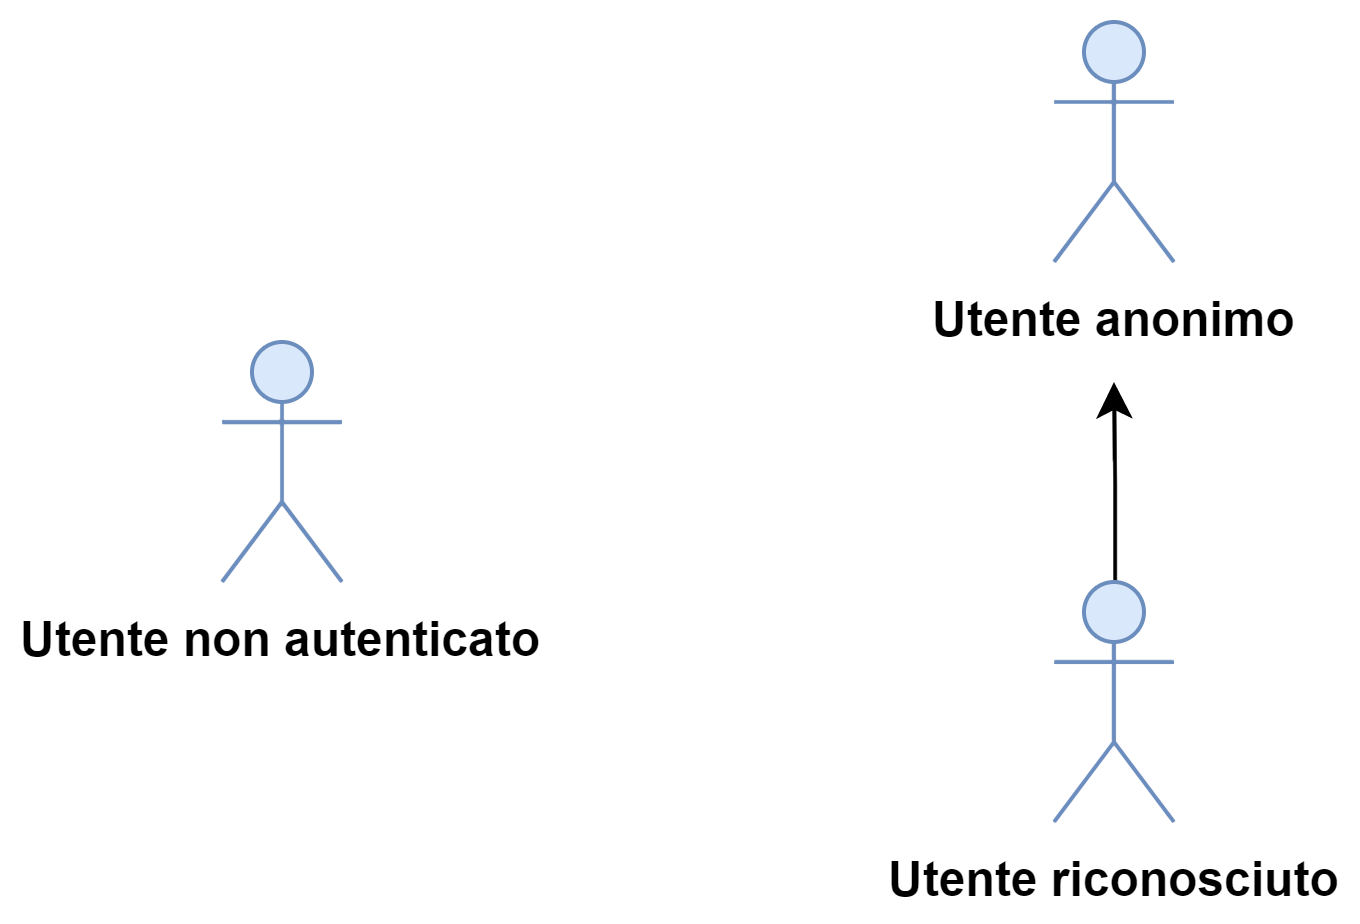
\includegraphics[scale=0.8]{Sezioni/UseCase/Immagini/Utenti.png}
    \caption{Gerarchia degli utenti}
\end{figure}

\paragraph{Utente non autenticato}
Utente non ancora autenticato all'applicazione che può avere o non avere le credenziali per autenticarsi.
\paragraph{Utente anonimo}
Utente autenticato che può venire tracciato all'interno di una \glo{organizzazione} senza fornire dettagli sulla propria identità.
\paragraph{Utente riconosciuto}
Utente autenticato che è attualmente tracciato all'interno di una precisa \glo{organizzazione} fornendo dettagli sulla propria identità.
L'utente si è precedentemente autenticato presso l'\glo{organizzazione} tramite LDAP.



\subsubsection{Attori Amministratori}
\begin{figure}[h]
  \centering
    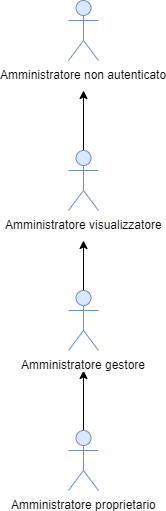
\includegraphics[scale=0.8]{Sezioni/UseCase/Immagini/Amministratori.png}
    \caption{Gerarchia degli amministratori}
\end{figure}


\paragraph{Amministratore non autenticato}
Amministratore non ancora autenticato nel sistema che ha già le credenziali per autenticarsi.
\paragraph{Amministratore autenticato}
Amministratore che si è autenticato nel sistema.
\paragraph{Amministratore proprietario}
Amministratore autenticatosi con il ruolo di proprietario dell'\glo{organizzazione}.
Si trova al gradino più alto della gerarchia degli amministratori e dispone delle seguenti funzioni:
\begin{itemize}
\item Gestire l'\glo{organizzazione}, ovvero modificarne i dati (come nome, descrizione, ecc.) e le superfici geografiche per il \glo{tracciamento} degli utenti;
\item Gestire gli amministratori, cioè la loro nomina, rimozione e modifica dei privilegi;
\item Monitorare gli accessi;
\item Eliminare l'\glo{organizzazione}.
\end{itemize}
Il proprietario dell'\glo{organizzazione} può nominare altri amministratori.
\paragraph{Amministratore gestore}
Amministratore autenticatosi con il ruolo di gestore. 
Si trova al secondo gradino della gerarchia degli amministratori e dispone delle seguenti funzioni:
\begin{itemize}
\item Gestire l'\glo{organizzazione};
\item Monitorare gli accessi.
\end{itemize}
\paragraph{Amministratore visualizzatore}
Amministratore autenticatosi con il ruolo di visualizzatore.
Escludendo l'amministratore non autenticato si trova all'ultimo gradino della gerarchia degli amministratori e può compiere solo la seguente funzione:
\begin{itemize}
\item Monitorare gli accessi.
\end{itemize}

%Alternativa in caso esista una gerarchia a 3 livelli




\clearpage
\subsection{Elenco casi d'uso}
\setcounter{secnumdepth}{0}
\input{sezioni/UseCase/UCA1.tex}
\input{sezioni/UseCase/UCA2.tex}
\input{sezioni/UseCase/UCA3.tex}
\input{sezioni/UseCase/UCA4.tex}
%\input{sezioni/UseCase/UCA5.tex}
%\input{sezioni/UseCase/UCA6.tex}
\input{sezioni/UseCase/UCA7.tex}
\input{sezioni/UseCase/UCA8.tex}
\input{sezioni/UseCase/UCS1.tex}
\input{sezioni/UseCase/UCS2.tex}
\input{sezioni/UseCase/UCSModificaDatiOrg.tex}
\input{sezioni/UseCase/UCS6.tex}
\input{sezioni/UseCase/UCS7.tex}

\clearpage

\setcounter{secnumdepth}{3}
\section{Requisiti}
\renewcommand{\o}{Obbligatorio}
\renewcommand{\d}{Desiderabile}
\newcommand{\op}{Opzionale}

Rappresentano dei requisiti che deve soddisfare il prodotto che si vuole realizzare.\\
I requisiti saranno organizzati in forma tabellare.\\
La tabella avrà le seguenti tre colonne:
\begin{itemize}
	\item Codice identificativo
	\item Classificazione
	\item Descrizione
	\item Fonti
\end{itemize}
\paragraph{Codice identificativo dei requisiti}\mbox{}\\
Ogni requisito sarà strutturato come segue:
\begin{itemize}
	\item Identificativo: \textbf{R[Importanza][Tipologia][Codice]}\\
Dove:
\begin{itemize}
		\item \textbf{Importanza:}
		\begin{itemize}
			\item \textbf{1}: requisito obbligatorio, ovvero irrinunciabile per almeno uno degli stakeholder
			\item \textbf{2}: requisito desiderabile, ovvero non strettamente necessario ma che porta valore aggiunto riconoscibile
			\item \textbf{3}: requisito opzionale, ovvero relativamente utile oppure contrattabile più avanti nel progetto
		\end{itemize}
		\item \textbf{Tipologia:}
		\begin{itemize}
			\item \textbf{F}: funzionale, definisce una funzione di un sistema di uno o più dei suoi componenti
			\item \textbf{Q}: qualitativo, definisce un requisito per garantire la qualità per un certo aspetto del progetto
			\item \textbf{P}: prestazionale, definisce un requisito che garantisce efficienza prestazionale nel prodotto
			\item \textbf{V}: vincolo, definisce un requisito volto a far rispettare un dato vincolo
		\end{itemize}
		\item \textbf{Codice:}\\
		Composto da:
		\begin{itemize}
			\item A*\ap{I} se il requisito proviene da un caso d'uso dell'applicazione, dove *\ap{I} sarà composto da: il numero del caso d'uso (lato app) kite-level di provenienza, un punto e il numero progressivo univoco
			\item S*\ap{II} se il requisito proviene da un caso d'uso del server, dove *\ap{II} sarà composto da: il numero del caso d'uso (lato server) kite-level di provenienza, un punto e il numero progressivo univoco
			\item C*\ap{III} se il requisito proviene dal capitolato, dove *\ap{III} sarà il numero progressivo univoco
			\item V*\ap{IV} se il requisito proviene da un verbale, dove *\ap{IV} inizierà con il numero che indica il verbale da cui proviene il requisito; il numero si calcola a partire da 1, che sarà associato al primo verbale redatto (in ordine temporale). Infine vi sarà un punto seguito dal numero progressivo
			\item I*\ap{V} se il requisito proviene da una decisione presa internamente al gruppo, dove *\ap{V} sarà un numero progressivo
		\end{itemize}
\end{itemize}
	\item \textbf{Descrizione}: descrizione sintetica ma al contempo esaustiva del requisito.
	\item \textbf{Classificazione}: informazione ridondante, sotto forma testuale, dell’importanza del requisito. Facilita la lettura dei requisiti.
	\item \textbf{Fonti}: definisce da dove deriva il requisito. I requisiti vengono raccolti da una o più fonti tra quelle citate di seguito:
	\begin{itemize}
		\item \textbf{Capitolato}: requisito individuato dalla lettura e/o analisi del capitolato
		\item \textbf{Interno}: requisito che gli analisti hanno ritenuto opportuno aggiungere
		\item \textbf{Caso d’uso}: il requisito è derivato da uno o più casi d’uso. Riportare anche il/i codice/i identificativo/i del/i caso/i d’uso.
		\item \textbf{Verbale}: requisito derivato in seguito ad una richiesta di chiarimento con il committente. Riportare il nome del documento del verbale da cui deriva il requisito in questione.		
	\end{itemize}
\end{itemize}

\subsection{Requisiti funzionali}
{
\rowcolors{2}{grigetto}{white}
\renewcommand{\arraystretch}{1.5}
\centering
\begin{longtable}{ c C{6.5cm} c c}
\caption{Tabella dei Requisiti funzionali}\\
\rowcolor{darkblue}
\textcolor{white}{\textbf{Identificativo}} & \textcolor{white}{\textbf{Descrizione}} & \textcolor{white}{\textbf{Classificazione}} & \textcolor{white}{\textbf{Fonti}}\\	
\endfirsthead
\rowcolor{darkblue}
\textcolor{white}{\textbf{Identificativo}} & \textcolor{white}{\textbf{Descrizione}} & \textcolor{white}{\textbf{Classificazione}} & \textcolor{white}{\textbf{Fonti}}\\
\endhead

R1FI1 & Un utente non autenticato non può effettuare alcuna azione a meno di autenticazione e registrazione. & \o & Interno\\

R1FA1.1 & L'autenticazione da parte di un utente non autenticato necessita di e-mail. & \o & UCA 1.1.1 Interno\\

R1FA1.2 & L'autenticazione da parte di un utente non autenticato necessita di password. & \o & UCA 1.1.2 Interno\\

R1FA8.1 & L'autenticazione viene negata qualora l'utente non autenticato tenti di autenticarsi con delle credenziali errate. Viene inoltre visualizzato un messaggio d'errore. & \o & UCA 8.1.4 Interno\\

R1FA1.3 & La registrazione da parte di un utente non autenticato necessita di e-mail. & \o & UCA 1.2.1 Interno\\

R1FA8.2 & Il processo di registrazione dell'utente non autenticato viene negato qualora l'e-mail inserita fosse già registrata nel sistema. Viene visualizzato inoltre un messaggio d'errore. & \o & UCA 8.1.1 Interno\\

R1FA1.4 & La registrazione da parte di un utente non autenticato necessita di password. & \o & UCA 1.2.2 Interno\\

R1FA1.5 & La registrazione da parte di un utente non autenticato necessita di conferma della password. & \o & UCA 1.2.3 Interno\\

R1FA1.6 & Durante la registrazione viene chiesto all'utente non autenticato di accettare le condizioni generali d'uso. & \o & UCA 1.2.4 Interno\\

R1FA1.7 & Qualora l'utente non autenticato dovesse rifiutare le condizioni generali d'uso allora la registrazione non può essere terminata correttamente.  & \o & UCA 1.2.4 Interno\\

R2FA1.8 & L'utente non autenticato deve essere in grado di effettuare il reset della password qualora se la fosse dimenticata. & \d & UCA 1.3 Interno\\

R2FA1.9 & Il reset della password da parte dell'utente non autenticato richiede l'e-mail del proprio account. & \d & UCA 1.3.1 Interno\\

R2FA1.10 & Il reset della password da parte dell'utente non autenticato richiede l'e-mail di recupero per effettuare il cambio password. & \d & UCA 1.3.2 Interno\\

R2FA1.11 & Il reset della password da parte dell'utente non autenticato richiede la nuova password. & \d & UCA 1.3.3 Interno\\

R2FA1.12 & Il reset della password da parte dell'utente non autenticato richiede la conferma della nuova password. & \d & UCA 1.3.4 Interno\\

R1FA8.3 & Il processo di autenticazione viene negato qualora la password inserita non sia abbastanza sicura. Viene visualizzato inoltre un messaggio d'errore. & \o & UCA 8.1.2 Interno\\

R1FA8.4 & Il processo di registrazione viene negato se password e conferma password inserita non combaciano. Viene visualizzato inoltre un messaggio d'errore. & \o & UCA 8.1.3 Interno\\


%PERIN

R1FA2.1 & L'utente anonimo e riconosciuto deve essere in grado di effettuare il logout. & \o & UCA 2 Interno\\

R1FA3.1 & L'utente anonimo può gestire la propria lista delle organizzazioni. & \o & UCA 3 Interno\\

R1FA3.2 & L'utente anonimo deve poter essere in grado di scaricare la lista di tutte le organizzazioni. & \o & UCA 3.1 Capitolato \\

R1FA8.5 & Qualora fallisca lo scaricamento della lista delle organizzazioni deve venire visualizzato un messaggio d'errore che lo informa di tale evento. & \o & UCA 8.3.1 Interno \\

R1FA3.3 & L’utente anonimo deve poter essere in grado di gestire la propria lista delle organizzazioni preferite. & \o & UCA 3.2 Interno \\

R1FA3.4 & L’utente anonimo può inserire una organizzazione presente nella lista delle organizzazioni, nella propria lista delle organizzazioni preferite. & \o & UCA 3.2.1 Interno \\

R1FA3.5 & Qualora l’utente anonimo inserisca un'organizzazione nella propria lista delle organizzazioni preferite che richiede autenticazione con credenziali LDAP, deve autenticarsi con credenziali LDAP. & \o & UCA 3.2.2 Capitolato\\

R1FA3.6 & L’utente anonimo può rimuovere una organizzazione presente nella propria lista delle organizzazioni preferite. & \o & UCA 3.2.3 Interno \\

R1FA8.6 & Qualora non sia memorizzata nessuna lista delle organizzazioni nel dispositivo, viene informato l’utente di questo fatto. & \o & UCA 8.3.2 Interno \\

R1FA3.7 & L’utente anonimo ha la possibilità di aggiornare la lista delle organizzazioni. & \o & UCA 3.3 Interno \\

R1FA3.8 & L’utente anonimo può aggiornare la lista delle organizzazioni tramite refresh manuale. & \o & UCA 3.3.1 Interno \\

R1FA3.9 & L’utente  anonimo può aggiornare la lista delle organizzazioni tramite temporizzazione. & \o & UCA 3.3.2 Interno \\

R1FA3.10 & L’utente anonimo può visualizzare la lista delle organizzazioni. & \o & UCA 3.4 Interno \\

R2FA3.11 & L’utente anonimo ha la possibilità di visualizzare la lista delle organizzazioni ordinate alfabeticamente, dalla A alla Z. & \d & UCA 3.4.1 Interno \\

R2FA3.12 & L’utente anonimo ha la possibilità di visualizzare la lista delle organizzazioni ordinate secondo politica \glo{FIFO}. & \d & UCA 3.4.2 Interno \\

R3FA3.13 & L’utente anonimo ha la possibilità di visualizzare la lista delle organizzazioni che permettono il tracciamento anonimo. & \op & UCA 3.4.3 Interno \\

R3FA3.14 & L’utente anonimo ha la possibilità di visualizzare la lista delle organizzazioni che permettono il \glo{tracciamento autenticato}. & \op & UCA 3.4.4 Interno \\

R1FA3.15 & L’utente anonimo può effettuare ricerche personalizzate per cercare le organizzazioni presenti nella lista delle organizzazioni. & \o & UCA 3.5 Interno\\

R2FA3.16 & L’utente anonimo può ricercare organizzazioni presenti nella lista delle organizzazioni appartenenti alla nazione indicata dall’utente. & \d & UCA 3.5.1 Interno \\

R1FA3.17 & L’utente anonimo può ricercare organizzazioni presenti nella lista delle organizzazioni che hanno nel nome una sotto-stringa scelta dall'utente. & \o & UCA 3.5.2 Interno \\

R2FA3.18 & L’utente anonimo può ricercare organizzazioni presenti nella lista delle organizzazioni appartenenti alla città indicata dall’utente. & \d & UCA 3.5.3 Interno \\

R1FA4.1 & L’utente riconosciuto deve poter inserire la modalità di tracciamento che preferisce. & \o & UCA 4 Capitolato \\

R1FA4.2 & L’utente riconosciuto può selezionare la modalità di tracciamento anonimo. & \o & UCA 4.1 Capitolato \\

R1FA4.3 & L’utente riconosciuto può selezionare la modalità di \glo{tracciamento autenticato}. & \o & UCA 4.2 Capitolato \\

R2FA5.1 & L’utente anonimo ha la possibilità di visualizzare il proprio storico degli accessi. & \d & UCA 5 Capitolato \\

R2FA5.2 & L’utente anonimo ha la possibilità di visualizzare il proprio storico degli accessi presso una organizzazione. & \d & UCA 5.1 Capitolato \\

R2FA5.3 & L'utente anonimo nella visualizzazione del proprio storico degli accessi nell'organizzazione visualizza la data per ogni accesso di quando è stato fatto. & \d & UCA 5.1.4 \\

R2FA5.4 & L'utente anonimo nella visualizzazione del proprio storico degli accessi nell'organizzazione visualizza il luogo per ogni accesso di quando è stato fatto. & \d & UCA 5.1.4 \\

R2FA5.5 & L'utente anonimo nella visualizzazione del proprio storico degli accessi nell'organizzazione visualizza il tempo trascorso per ogni accesso. & \d & UCA 5.1.4 \\

R2FA5.6 & L’utente anonimo ha la possibilità di visualizzare il proprio storico degli accessi presso un luogo dell’organizzazione. & \d & UCA 5.2 Capitolato\\

R2FA5.7 & L'utente anonimo nella visualizzazione del proprio storico degli accessi nel luogo dell'organizzazione visualizza la data per ogni accesso di quando è stato fatto. & \d &  UCA 5.2.4 \\

R2FA5.8 & L'utente anonimo nella visualizzazione del proprio storico degli accessi nel luogo dell'organizzazione visualizza il luogo per ogni accesso di quando è stato fatto. & \d &  UCA 5.2.4 \\

R2FA5.9 & L'utente anonimo nella visualizzazione del proprio storico degli accessi nel luogo dell'organizzazione visualizza il tempo trascorso per ogni accesso. & \d &  UCA 5.2.4 \\

R2FA5.10 & L’utente anonimo può visualizzare la propria lista degli accessi in una organizzazione ordinata per data decrescente. & \d & UCA 5.4.1 \\

R2FA5.11 & L’utente anonimo può visualizzare la propria lista degli accessi in una organizzazione ordinata per data crescente. & \d & UCA 5.4.2 \\

R3FA5.12 & L’utente anonimo può effettuare una ricerca degli accessi presso un'organizzazione in un giorno specifico. & \op & UCA 5.5 \\

R2FA5.13 & L’utente anonimo può visualizzare la propria lista degli accessi presso un luogo dell’organizzazione ordinata per data decrescente. & \d & UCA 5.4.1 \\

R2FA5.14 & L’utente anonimo può visualizzare la propria lista degli accessi presso un luogo dell’organizzazione ordinata per data crescente. & \d & UCA 5.4.2 \\

R3FA5.15 & L’utente anonimo può effettuare una ricerca degli accessi presso un luogo dell’organizzazione in un giorno specifico. & \op & UCA 5.5 \\

R2FA5.16 & L’utente anonimo se si trova all’interno dell’organizzazione ha la possibilità di visualizzare il tempo passato all’interno dall'ultimo ingresso effettuato. & \d & UCA 5.1.5 Capitolato \\

R2FA5.17 & L’utente anonimo se si trova all’interno dell’luogo dell’organizzazione ha la possibilità di visualizzare il tempo passato all’interno dall'ultimo ingresso effettuato. & \d & UCA 5.2.5 Capitolato \\

R2FA8.5 & Qualora non ci sono accessi effettuati presso l'organizzazione selezionata, l'utente anonimo deve essere informato di ciò. & \d & UCA 8.5.1 Interno \\

R2FA8.6 & Qualora non ci sono accessi effettuati presso il luogo selezionato, l'utente anonimo deve essere informato di ciò. & \d & UCA 8.5.2 Interno \\

R1FA6.1 & L’utente che effettua un movimento nell’organizzazione deve essere notificato della sua azione e il movimento deve essere memorizzato nel sistema. & \o & UCA 6.1 Capitolato \\

R1FA6.2 & L’utente che effettua un movimento nell’organizzazione, deve essere notificato della sua azione. & \o & UCA 6.1.1 \\

R1FA6.3 & L’utente che effettua un movimento in un luogo all'interno di una organizzazione, deve essere notificato della sua azione. & \o & UCA 6.2.1 \\

R1FA6.4 & L’utente che effettua un movimento in un luogo di un'organizzazione deve essere notificato della sua azione e il movimento deve essere memorizzato nel sistema. & \o & UCA 6.2 Capitolato \\

R1FA8.7 & Qualora non vengano memorizzate le informazioni necessarie per la registrazione del movimento effettuato dall’utente, deve essere notificato tale evento all’utente. & \o & UCA 8.6.1 \\

%Cisotto

R1FA7.1 & L'utente anonimo deve avere la possibilità di autenticarsi con le credenziali aziendali in un'organizzazione che richiede il tracciamento riconosciuto. & \o & UCA 7 Capitolato \\

R1FA8.8 & Qualora le credenziali LDAP aziendali inserite dall'utente non fossero riconosciute dal server aziendale associato viene mostrato un messaggio d'errore. & \o & UCA 8.7.1 Interno \\

R1FA7.2 & L'utente anonimo deve avere la possibilità di inserire il nome utente durante l'autenticazione con le credenziali LDAP aziendali. & \o & UCA 7.1.1 Interno \\

R1FA7.3 & L'utente anonimo deve avere la possibilità di inserire la password durante l'autenticazione con le credenziali LDAP aziendali. & \o & UCA 7.1.2 Interno \\

R1FI2 & Un utente non autenticato non può effettuare alcuna azione a meno di autenticazione. & \o & Interno \\

R1FS1.1 & L’autenticazione da parte di un amministratore necessita di e-mail. & \o & UCS 1.1.1 Interno\\

R1FS10.1 & L’autenticazione viene negata qualora l'amministratore tenti di autenticarsi con delle credenziali errate. & \o & UCS 10.1.1 Interno \\

R1FS10.2 & Qualora l'amministratore tenti di autenticarsi con le credenziali errate viene visualizzato un messaggio d’errore. & \o & UCS 10.1.1 Interno \\

R1FS1.2 & L’autenticazione da parte di un amministratore necessita di password. & \o & UCS 1.1.2 Interno\\

R2FS1.3 & L'utente non autenticato deve essere in grado di effettuare il reset della password qualora se la fosse dimenticata. & \d & UCS 1.3 Interno\\

R2FS1.4 & Il reset della password dell'utente non autenticato richiede l'e-mail. & \d & UCS 1.3.1 Interno \\

R2FS1.5 & Il reset della password dell'utente non autenticato richiede l'e-mail di recupero per il reset della password. & \d & UCS 1.3.2 Interno \\

R2FS1.6 & Il reset della password dell'utente non autenticato richiede la nuova password. & \d & UCS 1.3.3 Interno \\

R2FS1.7 & Il reset della password dell'utente non autenticato richiede la conferma della password. & \d & UCS 1.3.4 Interno \\

R1FS2.1 & L'amministratore deve essere in grado di effettuare il logout. & \o & UCS 2 Interno\\

R1FC3 & L'amministratore visualizzatore deve poter visualizzare le organizzazioni disponibili. & \o & Capitolato\\

R1FI3 & Deve venire mostrato il nome dell'organizzazione durante la sua visualizzazione da parte di un amministratore. & \o & Interno\\

R2FI4 & Deve venire mostrata l'immagine dell'organizzazione durante la sua visualizzazione da parte di un amministratore. & \d & Interno\\

R1FS3.1 & L'amministratore visualizzatore deve poter selezionare un'organizzazione tra quelle da lui visualizzate. & \o & UCS 3 Interno\\

R1FI5 & Deve venire mostrato il nome dell'organizzazione selezionata durante la sua visualizzazione da parte di un amministratore. & \o & Interno\\

R2FI6 & Deve venire mostrata l'immagine dell'organizzazione selezionata durante la sua visualizzazione da parte di un amministratore. & \d & Interno\\

R2FI7 & Deve venire mostrata la descrizione dell'organizzazione selezionata durante la sua visualizzazione da parte di un amministratore. & \d & Interno\\

R1FI8 & Deve venire mostrato l'indirizzo dell'organizzazione selezionata durante la sua visualizzazione da parte di un amministratore. & \o & Interno\\


R1FS4.1 & L'amministratore gestore deve poter modificare il nome dell'organizzazione. & \o & UCS 4.1.1 Interno\\

R2FS4.2 & L'amministratore gestore deve poter modificare l'immagine dell'organizzazione. & \d & UCS 4.1.2 Interno\\

R2FS4.3 & L'amministratore gestore deve poter modificare la descrizione dell'organizzazione. & \d & UCS 4.1.3 Interno\\

R1FS4.4 & L'amministratore gestore deve poter modificare l'indirizzo dell'organizzazione. & \o & UCS 4.1.4 Interno\\

R1FS4.5 & L'amministratore gestore deve poter modificare l'indirizzo IP dell'organizzazione. & \o & UCS 4.1.5 Interno\\

R1FS10.3 & Se il nome dell'organizzazione inserito dall'amministratore non rispetta i vincoli imposti viene mostrato un messaggio d'errore. & \o & UCS 10.4.2\\

R1FS10.4 & Se il nome dell'organizzazione inserito dall'amministratore dovesse essere già presente nel sistema e associato ad un'altra organizzazione viene mostrato un messaggio d'errore. & \o & UCS 10.4.3\\

R2FS10.5 & Se l'immagine dell'organizzazione selezionata dall'amministratore non rispetta i vincoli imposti viene mostrato un messaggio d'errore. & \d & UCS 10.4.4\\

R2FS10.6 & Se la descrizione dell'organizzazione inserita dall'amministratore non rispetta i vincoli imposti viene mostrato un messaggio d'errore. & \d & UCS 10.4.5\\

R1FS10.7 & Se l'indirizzo dell'organizzazione inserito dall'amministratore non rispetta i vincoli imposti viene mostrato un messaggio d'errore. & \o & UCS 10.4.6\\

R1FS10.8 & Se l'indirizzo URL non è valido viene mostrato un messaggio d'errore. & \o & UCS 10.4.7\\

R1FS4.6 & L'amministratore proprietario deve avere la possibilità di inviare la richiesta di eliminazione per un'organizzazione. & \o & UCS 4.2 Capitolato\\

R3FS4.7 & L'amministratore proprietario deve poter inserire una motivazione per la richiesta di eliminazione dell'organizzazione. & \op & UCS 4.2.1 Interno \\

R1FS4.8 & L'amministratore gestore deve poter annullare le modifiche che sta apportando. & \o & UCS 4.3 Interno\\



% Drago

R1FS5.1 & L'amministratore gestore deve poter modificare il perimetro di \glo{tracciamento} dell'\glo{organizzazione}. & \o & UCS 5.1 Capitolato\\

R1FS10.9 & La modifica del perimetro dell'organizzazione viene negata qualora l'amministratore selezioni un area che non rispetta i vincoli imposti. Viene visualizzato un messaggio di errore. & \o & UCS 10.5.1 Capitolato \\

R1FS5.2 & L'amministratore gestore deve essere in grado di creare dei nuovi luoghi di tracciamento nell'organizzazione. & \o & UCS 5.2 Capitolato\\

R1FS5.3 & L'amministratore gestore deve essere in grado di modificare i luoghi di tracciamento dell'organizzazione. & \o & UCS 5.3 Capitolato\\

R1FS10.10 & La creazione di nuovi luoghi e la modifica dell'area di tracciamento di essi vengono negati qualora l'amministratore selezioni un area che fuoriesce dal perimetro. Viene visualizzato un messaggio di errore. & \o & UCS 10.5.2 Capitolato \\

R1FS5.4 & L'amministratore gestore deve essere in grado di eliminare i luoghi di tracciamento dell'organizzazione. & \o & UCS 5.4 Capitolato\\

R1FS5.5 & L'amministratore gestore deve essere in grado di selezionare un'area geografica per il tracciamento del luogo scelto. & \o & UCS 5.5 Capitolato\\

R1FS5.6 & L'amministratore gestore può scegliere l'area di tracciamento tramite l'inserimento delle coordinate geografiche. & \o & UCS 5.5.1 Capitolato\\

R2FS5.7 & L'amministratore gestore può scegliere l'area di tracciamento tramite Google Maps API. & \d & UCS 5.5.2 Interno\\

R1FS5.9 & L'amministratore deve poter inserire un nome per il nuovo luogo di tracciamento. & \o & UCS 5.2.1 Interno\\

R1FS6.1 & L'amministratore può monitorare l'organizzazione visualizzando il numero di utenti anonimi presenti nell'organizzazione. & \o & UCS 6 Capitolato\\

R1FS6.2 & L'amministratore visualizzatore può monitorare l'organizzazione visualizzando il numero di utenti anonimi presenti in un specifico luogo dell'organizzazione. & \o & UCS 6.1 Capitolato\\

R1FS6.3 & L'amministratore visualizzatore ha la possibilità di ritornare al monitoraggio dell'organizzazione in generale dal monitoraggio di un luogo specifico. & \o & UCS 6.1.1 Interno\\

R1FS7.1 & L'amministratore visualizzatore può monitorare gli accessi effettuati dagli utenti riconosciuti. & \o & UCS 7 Capitolato\\

R1FS7.2 & L'amministratore visualizzatore può monitorare gli accessi effettuati presso una organizzazione da un specifico utente riconosciuto visualizzandone il nome, il cognome, l'orario di accesso, di uscita e il tempo di permanenza. & \o & UCS 7.1.4 Capitolato\\

R2FS7.3 & L’amministratore visualizzatore può filtrare la lista degli accessi presso una organizzazione di un utente riconosciuto per data decrescente. & \d & UCS 7.4.1 Interno \\

R2FS7.4 & L’amministratore visualizzatore può filtrare la lista degli accessi presso una organizzazione  di un utente riconosciuto per data crescente. & \d & UCS 7.4.2 Interno \\

R2FS7.5 & L'amministratore visualizzatore può monitorare gli accessi presso una organizzazione filtrandoli in base a una data precisa. & \d & UCS 7.5 Interno\\

R1FS7.6 & L'amministratore visualizzatore può monitorare gli accessi effettuati presso un luogo all'interno di una organizzazione da un specifico utente riconosciuto visualizzandone il nome, il cognome e l'orario di accesso. & \o & UCS 7.2.4 Capitolato\\

R2FS7.7 & L’amministratore visualizzatore può filtrare la lista degli accessi presso un luogo di un'organizzazione di un utente riconosciuto per data decrescente. & \d & UCS 7.4.1 Interno \\

R2FS7.8 & L’amministratore visualizzatore può filtrare la lista degli accessi presso un luogo di un'organizzazione di un utente riconosciuto per data crescente. & \d & UCS 7.4.2 Interno \\

R2FS7.9 & L'amministratore visualizzatore può monitorare gli accessi presso un luogo di un'organizzazione filtrandoli in base a una data precisa. & \d & UCS 7.5 Interno\\

R2FS8.1 & L'amministratore visualizzatore può ricevere un report tabellare degli accessi ai luoghi dell'organizzazione. & \o & UCS 8 Capitolato\\

R2FS8.2 &  Tabella delle entrate e uscite degli utenti nei luoghi dell'organizzazione generabile dall'amministratore visualizzatore di un organizzazione a \glo{tracciamento autenticato}. & \o & UCS 8.1.1 Capitolato\\

R2FS8.3 & Tabella delle ore spese dagli utenti nei luoghi dell'organizzazione generabile dall'amministratore visualizzatore di un organizzazione a \glo{tracciamento autenticato}. & \o & UCS 8.1.2 Capitolato\\

R2FS8.4 & Tabella contenente il numero degli utenti e il totale delle ore passate da essi nei luoghi dell'organizzazione generabile dall'amministratore visualizzatore di un organizzazione a \glo{tracciamento autenticato} o anonimo. & \o & UCS 8.1.3 Capitolato\\

%Cisotto

R1FS9.1 & L'amministratore proprietario ha la possibilità di entrare nella sezione di gestione degli amministratori (per la nomina, eliminazione e modifica dei privilegi ad altri amministratori). & \o & UCS 9 Capitolato \\

R1FI9 & L'amministratore proprietario ha la possibilità di visualizzare gli amministratori da esso nominati una volta entrato nella gestione degli amministratori. & \o & Interno \\

R1FI10 & La visualizzazione di un amministratore deve mostrare la sua e-mail. & \o & Interno \\

R1FI11 & La visualizzazione di un amministratore deve mostrare i suoi privilegi. & \o & Interno \\

R1FS9.2 & L'amministratore proprietario ha la possibilità di nominare un nuovo amministratore. & \o & UCS 9.1 Capitolato\\

R1FS9.3 & L'amministratore proprietario deve poter inserire un'e-mail per il nuovo amministratore da nominare. & \o & UCS 9.1.1 Interno\\

R1FS10.11 & Viene mostrato un messaggio d'errore qualora l'e-mail del nuovo amministratore da nominare risulti già registrata nel sistema. & \o & UCS 10.9.1 Interno\\

R1FS10.12 & Viene mostrato un messaggio d'errore qualora la password del nuovo amministratore da nominare risulti troppo debole. & \o & UCS 10.9.2 Interno\\

R1FS10.13 & Viene mostrato un messaggio d'errore qualora la password non combaci con la conferma password del nuovo amministratore da nominare. & \o & UCS 10.9.3 Interno\\

R1FS9.4 & L'amministratore proprietario deve poter inserire una nuova password per il nuovo amministratore da nominare. & \o & UCS 9.1.2 Interno\\

R1FS9.5 & L'amministratore proprietario deve poter inserire la conferma della nuova password per il nuovo amministratore da nominare. & \o & UCS 9.1.3 Interno\\

R1FS9.6 & L'amministratore proprietario deve poter selezionare i privilegi per il nuovo amministratore da nominare. & \o & UCS 9.1.4 Interno\\

R1FS9.7 & L'amministratore proprietario ha la possibilità di eliminare un amministratore togliendogli i permessi di amministrazione dell'organizzazione. & \o & UCS 9.2 Capitolato\\

R1FS9.8 & L'amministratore proprietario ha la possibilità di inserire la e-mail dell'account amministratore da eliminare. & \o & UCS 9.2.1 Interno\\

R1FS10.14 & Viene mostrato un messaggio d'errore qualora l'e-mail dell'amministratore da eliminare inserita non risulti registrata nel sistema. & \o & UCS 10.9.4 Interno\\

R1FS9.9 & L'amministratore proprietario ha la possibilità di modificare i privilegi di un amministratore. & \o & UCS 9.3 Interno\\

R1FS9.10 & L'amministratore proprietario ha la possibilità di inserire la e-mail dell'account amministratore a cui desidera modificare i privilegi. & \o & UCS 9.3.1 Interno\\

R1FS10.15 & Viene mostrato un messaggio d'errore qualora l'e-mail dell'amministratore a cui si vuole modificare i privilegi non risulti registrata nel sistema. & \o & UCS 10.9.4 Interno\\

R1FS9.11 & L'amministratore proprietario ha la possibilità annullare le modifiche che sta apportando agli amministratori. & \o & UCS 9.4 Interno\\

R1FS9.12 & L'amministratore proprietario ha la possibilità di nominare un account già presente nel sistema come amministratore della propria organizzazione & \o & UCS 9.5 Interno\\

R1FS9.13 & L'amministratore proprietario deve poter inserire un'e-mail per il nuovo amministratore da nominare. & \o & UCS 9.5.1 Interno\\

R1FS9.14 & L'amministratore proprietario deve poter selezionare i privilegi per il nuovo amministratore da nominare. & \o & UCS 9.5.2 Interno\\

R1FS10.16 & L'amministratore gestore deve poter annullare le modifiche che stava apportando all'organizzazione. & \o & UCS 10.4.1\\

R1FS10.17 & L'amministratore gestore deve poter annullare la selezione della nuova area geografica per il tracciamento di un luogo o del perimetro dell'organizzazione. & \o & UCS 10.5.3 Interno\\

R2FS10.18 & Deve venir mostrato un errore qualora avvenisse un errore da parte del server sulla generazione del report tabellare. & \d & UCS 10.6.1 Interno\\

\end{longtable}
}
\subsection{Requisiti prestazionali}
{
\rowcolors{2}{grigetto}{white}
\renewcommand{\arraystretch}{1.5}
\centering
\begin{longtable}{ c C{8cm} c c}
\rowcolor{rossoep}
\textcolor{white}{\textbf{Identificativo}} & \textcolor{white}{\textbf{Descrizione}} & \textcolor{white}{\textbf{Classificazione}} & \textcolor{white}{\textbf{Fonti}}\\	
\endhead

R1PC1 & L'applicazione deve bilanciare nel miglior modo possibile il consumo della batteria & Obbligatorio & Capitolato\\

R1PC2 & Il rintracciamento deve avere una precisione sufficiente a certificare la presenza della persona all'interno degli edifici & Obbligatorio & Capitolato\\

%R1PC3 & Scalabilità orizzontale?? & Obbligatorio & Capitolato\\
\end{longtable}
}
\subsection{Requisiti qualitativi}
{
\rowcolors{2}{grigetto}{white}
\renewcommand{\arraystretch}{1.5}
\centering
\begin{longtable}{ c C{8cm} c c}
\rowcolor{darkblue}
\textcolor{white}{\textbf{Identificativo}} & \textcolor{white}{\textbf{Descrizione}} & \textcolor{white}{\textbf{Classificazione}} & \textcolor{white}{\textbf{Fonti}}\\	
\endhead

R1QI1 & Le norme e le metriche definite nei documenti \textit{NormeDiProgetto} e \textit{PianoDiQualifica} sono state rispettate. & Obbligatorio & Interno\\

R1QI2 & Deve essere prodotto un manuale utente. & Obbligatorio & Interno\\

R1QI3 & Deve essere prodotto un manuale amministratore. & Obbligatorio & Interno\\

R1QI4 & Il codice sorgente deve essere caricato in una repository su GitHub. & Obbligatorio & Interno\\

R1QI5 & La documentazione riguardante il software deve essere disponibile in lingua italiana. & Obbligatorio & Interno\\

R1QV1 & Si deve scegliere una licenza tra GNU\ap{G}, GPL\ap{G}, LGPL\ap{G} e MIT\ap{G}. & Obbligatorio & VE\_2019\_12\_16 \\

\end{longtable}
}
\renewcommand{\o}{Obbligatorio}
\renewcommand{\d}{Desiderabile}
\subsection{Requisiti di vincolo}
{
\rowcolors{2}{grigetto}{white}
\renewcommand{\arraystretch}{2}
\centering
\begin{longtable}{ c C{8cm} c c}
\rowcolor{darkblue}
\textcolor{white}{\textbf{Identificativo}} & \textcolor{white}{\textbf{Descrizione}} & \textcolor{white}{\textbf{Classificazione}} & \textcolor{white}{\textbf{Fonti}}\\	
\endhead

R1VC1.1 & Deve essere sviluppato un server back-end & \o & Capitolato \\
R1VC1.2 & Il server deve essere correlato di una UI\ap{G} per la gestione delle funzioni implementate& \o & Capitolato \\
R1VC1.3 & Deve essere sviluppata una applicazione mobile per sistemi operativi Android o IOS & \o & Capitolato \\
R1VC2.1 & Le comunicazioni di tracciamento tra applicazione cellulare e Server devono avvenire solo al momento d’ingresso ed uscita dai luoghi designati & \o & Capitolato \\
R2VC3.1 & Possibile utilizzo di Java\ap{G} (versioni 8 o superiori) per sviluppo Server back-end & \d & Capitolato \\
R2VC3.2 & Possibile utilizzo di Python\ap{G} per sviluppo server back-end & \d & Capitolato \\
R2VC3.3 & Possibile utilizzo di Nodejs\ap{G}per sviluppo server back-end & \d & Capitolato \\
R2VC4.1 & Possibile utilizzo di protocolli asincroni\ap{G} per le comunicazioni app mobile-server & Desiderato & Capitolato \\
R2VC5.1 & Possibile utilizzo del pattern di Publish/Subscriber\ap{G} & \d & Capitolato \\
R2VC6.1 & Possibile utilizzo dell’IAAS Kubernetes\ap{G} per la gestione della scalabilità orizzontale\ap{G}& \d & Capitolato \\
R2VC6.2 & Possibile utilizzo di PAAS\ap{G} per la gestione della scalabilità orizzontale\ap{G}& \d & Capitolato \\
R2VC6.3 & Possibile utilizzo di Openshift\ap{G} per la gestione della scalabilità orizzontale\ap{G}& \d & Capitolato \\
R2VC6.4 & Possibile utilizzo di Rancher\ap{G} per la gestione della scalabilità orizzontale\ap{G}& \d & Capitolato \\
R1VC7.1 & Il server deve esporre oltre a eventuali protocolli richiesti per l’interazione con il servizio, delle API Rest\ap{G} necessarie per permettere l’utilizzo applicativo, come alternativa alle API Rest\ap{G} è possibile utilizzare gRPC\ap{G} & \o & Capitolato \\
R2VC8.1 & Utilizzo di tecnologie network-GPS\ap{G} per il tracciamento della posizione & \d & Capitolato \\
R1VC8.2 & Si deve fornire un resoconto sulle scelte fatte e sui test effettuati relativi al tracciamento della posizione & \o & Capitolato \\
R1VC9.1 & Si deve correlare a tutte le componenti applicative dei test di unità e d’integrazione & \o & Capitolato \\
R1VC9.2 & Si deve testare tramite test end to end il sistema nella sua interezza & \o & Capitolato \\
R1VC9.3 & Devono essere effettuati test di carico per testare il corretto funzionamento della scalabilità & \o & Capitolato \\
R1VC9.4 & Si deve avere una copertura dei test maggiore o uguale al 80\% & \o & Capitolato \\
R1VC9.5 & Tutti i test effettuati devono essere correlati da un report & \o & Capitolato \\
R1VC10.1 & Deve essere scritta la documentazione relativa alle scelte implementative e progettuali con annessa motivazione & \o & Capitolato \\
R1VC10.2 & Deve essere scritta la documentazione relativa ai problemi aperti e eventuali soluzioni proposte da esplorare & \o & Capitolato \\
R2VC11.1 & Cifratura di tutte le comunicazioni fra App e Server & \d & Capitolato  \\
R1VC12.1 & Si deve utilizzare il protocollo LDAP per autenticare i singoli dipendenti e gli amministratori di una organizzazione per poter effettuare il tracciamento autenticato della posizione & \o & Capitolato \\	
R1VV1.1 & Deve essere garantita la privacy e quindi verificare che tutte le informazioni raccolte rispettino le GDPR\ap{G} & \o & VE\_2019\_12\_16 \\
R1VV1.2 & Le credenziali per accedere alla applicazione e le credenziali per accedere e autenticarsi in una organizzazione che richiede tracciamento autenticato devono essere diverse & \o & VE\_2019\_12\_16 \\
R1VV1.3 & I server LDAP delle organizzazioni che richiedono autenticazione devono essere esterni al sistema.  & \o & VE\_2019\_12\_16 \\
R1VV1.4 & Per gli utenti che non devono essere autenticati, si deve assegnare a loro un codice che ne certifichi la validità dell’ingresso o dell'uscita da un luogo in modo tale da non conoscere chi lo ha generato & \o & VE\_2019\_12\_16 \\
\end{longtable}
}

\section{Tracciamento}
\subsection{Tracciamento Fonte-Requisito}
{
\rowcolors{2}{grigetto}{white}
\renewcommand{\arraystretch}{1.5}
\centering
\begin{longtable}{ c C{4cm} c c}
\rowcolor{rossoep}
\textcolor{white}{\textbf{Fonte}} & \textcolor{white}{\textbf{Requisito}}\\	
\endhead

%% Requisiti funzionali

Interno & R1FI1\\

Interno & R1FA1.1\\

Interno & R1FA1.2\\

Interno & R1FA8.1\\

Interno & R1FA1.3\\

Interno & R1FA8.2\\

Interno & R1FA1.4\\

Interno & R1FA1.5\\

Interno & R1FA1.6\\

Interno & R1FA1.7\\

%%SEPARAZIONE

Interno & R2FA1.8\\

Interno & R1FA8.3\\

Interno & R1FA8.4\\

Interno & R1FA2\\

Interno & R1FA3.1\\

Capitolato & R1FA3.2\\

Interno & R1FA8.3\\

Interno & R1FA3.3\\

Interno & R1FA3.4\\

%% SEPARAZIONE

Capitolato & R1FA3.5\\

Interno & R1FA3.6\\

Interno & R1FA8.4\\

Interno & R1FA3.7\\

Interno & R1FA3.8\\

Interno & R1FA3.9\\

Interno & R1FA3.10\\

Interno & R1FA3.11\\

Interno & R1FA3.12\\

Interno & R1FA3.13\\

%% SEPARAZIONE

Interno & R1FA3.14\\

Interno & R1FA3.15\\

Interno & R1FA3.16\\

Interno & R1FA3.17\\

Interno & R1FA3.18\\

Capitolato & R1FA4.1\\

Capitolato & R1FA4.2\\

Capitolato & R1FA4.3\\

Capitolato & R2FA5.1\\

Capitolato & R2FA5.2\\

%% SEPARAZIONE

Interno & R2FA5.3\\

Interno & R2FA5.4\\

Interno & R2FA5.5\\

Capitolato & R2FA5.6\\

Interno & R2FA5.7\\

Interno & R2FA5.8\\

Interno & R2FA5.9\\

Interno & R2FA5.10\\

Interno & R2FA5.11\\

%% SEPARAZIONE

Interno & R2FA5.12\\

Interno & R2FA5.13\\

Interno & R2FA5.14\\

Interno & R3FA5.15\\

Capitolato & R2FA5.16\\

Capitolato & R2FA5.17\\

Interno & R2FA8.5\\

Interno & R2FA8.6\\

Capitolato & R2FA6.1\\

%% SEPARAZIONE

Interno & R2FA6.2\\

Interno & R2FA6.3\\

Interno & R2FA6.4\\

Capitolato & R2FA6.5\\

Capitolato & R2FA6.6\\

Capitolato & R2FA6.7\\

Capitolato & R2FA6.8\\

%% SEPARATORE

Interno & R2FA8.7\\

Interno & R2FA6.9\\

Capitolato & R1F7.1\\

Interno & R1F8.8\\

Interno & R1F7.2\\

Interno & R1F7.3\\

Interno & R1FI2\\

Interno & R1FS1.1\\

Interno & R1FS10.1\\

%% SEPARATORE

Interno & R1FS10.2\\

Interno & R1FS1.2\\

Interno & R2FS1.3\\

Interno & R1FS2.1\\

Capitolato & R1FC3\\

Interno & R1FI3\\

Interno & R2FI4\\

Interno & R1FS3.1\\

Interno & R1FI5\\

Interno & R2FI6\\

Interno & R2FI7\\

%% SEPARATORE

Interno & R1FI8\\

Interno & R1FS4.1\\

Interno & R1FS4.2\\

Interno & R2FS4.3\\

Interno & R2FS4.4\\

Interno & R2FS4.5\\

Interno & R2FS4.6\\

Interno & R1FS4.7\\

Interno & R1FS4.8\\

Interno & R1FS4.9\\

Interno & R1FS4.10\\

%% SEPARATORE

Interno & R1FS10.3\\

Interno & R1FS10.4\\

Interno & R2FS10.5\\

Interno & R2FS10.6\\

Interno & R1FS10.7\\

Interno & R1FS10.8\\

Capitolato & R1FS4.9\\

%% SEPARATORE

Interno & R3FS4.10\\

Interno & R1FS4.11\\

Capitolato & R1FS5.1\\

Capitolato & R1FA10.9\\

Capitolato & R1FS5.2\\

Capitolato & R1FS5.3\\

Capitolato & R1FS10.10\\

Capitolato & R1FS5.4\\

Capitolato & R1FS5.5\\

%% SEPARATORE

Capitolato & R1FS5.6\\

Interno & R2FS5.7\\

Interno & R1FS5.8\\

Capitolato & R1FS6.1\\

Capitolato & R1FS6.2\\

Capitolato & R1FS7.1\\

Capitolato & R1FS7.2\\

Interno & R2FS7.3\\

Interno & R2FS7.4\\

Interno & R2FS7.5\\

Capitolato & R1FS7.6\\

Capitolato & R1FS8.1\\

%% SEPARATORE

Capitolato & R1FS8.2\\

Capitolato & R1FS8.3\\

Capitolato & R1FS8.4\\

Capitolato & R1FS9.1\\

Interno & R1FI9\\

Interno & R1FI10\\

Interno & R1FI11\\

Capitolato & R1FS9.2\\

%% SEPARATORE

Interno & R1FS9.3\\

Interno & R1FS10.11\\

Interno & R1FS10.12\\

Interno & R1FS10.13\\

Interno & R1FS9.4\\

Interno & R1FS9.5\\

Interno & R1FS9.6\\

Capitolato & R1FS9.7\\

Interno & R1FS9.8\\

%% SEPARATORE

Interno & R1FS10.14\\

Interno & R1FS9.9\\

Interno & R1FS9.10\\

Interno & R1FS10.15\\

Interno & R1FS9.11\\

%% Requisiti funzionali

Capitolato & R1PC1\\

Capitolato & R1PC2\\

%% Requisiti qualitativi

Interno & R1QI1\\

Interno & R1QI2\\

Interno & R1QI3\\

Interno & R1QI4\\

Interno & R1QI5\\

VE\_2019\_12\_16 & R1QVE1\\

%% Requisiti di vincolo

Capitolato & R1VC1.1\\

Capitolato & R1VC1.2\\

Capitolato & R1VC1.3\\

Capitolato & R1VC2.1\\

Capitolato & R2VC3.1\\

Capitolato & R2VC3.2\\

Capitolato & R2VC3.3\\

Capitolato & R2VC4.1\\

Capitolato & R2VC5.1\\

%% SEPARATORE

Capitolato & R2VC6.1\\

Capitolato & R2VC6.2\\

Capitolato & R2VC6.3\\

Capitolato & R2VC6.4\\

Capitolato & R1VC7.1\\

Capitolato & R2VC8.1\\

Capitolato & R2VC8.2\\

Capitolato & R1VC9.1\\

Capitolato & R1VC9.2\\

Capitolato & R1VC9.3\\

Capitolato & R1VC9.4\\

Capitolato & R1VC9.5\\

Capitolato & R1VC10.1\\

Capitolato & R1VC10.2\\

Capitolato & R2VC11.1\\

Capitolato & R2VC12.1\\

%% SEPARATORE

VE\_2019\_12\_16 & R1VV1.1\\

VE\_2019\_12\_16 & R1VV1.2\\

VE\_2019\_12\_16 & R1VV1.3\\

VE\_2019\_12\_16 & R1VV1.4\\


\end{longtable}
}


\subsection{Tracciamento Caso d'uso-Requisito}
{
\rowcolors{2}{grigetto}{white}
\renewcommand{\arraystretch}{1.5}
\centering
\begin{longtable}{ c C{4cm} c c}
\rowcolor{rossoep}
\textcolor{white}{\textbf{Caso d'uso}} & \textcolor{white}{\textbf{Requisito}}\\	
\endhead

%% Requisiti funzionali

UCA 1.1.1 & R1FA1.1\\

UCA 1.1.2 & R1FA1.2\\

UCA 7 & R1FA7.1\\

UCA 1.2.1 & R1FA1.3\\

UCA 7.1.1 & R1FA7.2\\

UCA 1.2.2 & R1FA1.4\\

UCA 1.2.3 & R1FA1.5\\

UCA 1.2.4 & R1FA1.6\\

UCA 1.2.4 & R1FA1.7\\

%%SEPARAZIONE

UCA 1.3 & R2FA1.8\\

UCA 8.1.3 & R1FA8.3\\

UCA 8.1.3 & R1FA8.4\\

UCA 2 & R1FA2\\

UCA 3 & R1FA3.1\\

UCA 3.1 & R1FA3.2\\

UCA 8.1.3 & R1FA8.3\\

UCA 3.2 & R1FA3.3\\

UCA 3.2.1 & R1FA3.4\\

%% SEPARAZIONE

UCA 3.2.2 & R1FA3.5\\

UCA 3.2.3 & R1FA3.6\\

UCA 8.1.3 & R1FA8.4\\

UCA 3.3 & R1FA3.7\\

UCA 3.3.1 & R1FA3.8\\

UCA 3.3.2 & R1FA3.9\\

UCA 3.4 & R1FA3.10\\

UCA 3.4.1 & R1FA3.11\\

UCA 3.4.2 & R1FA3.12\\

UCA 3.4.3 & R1FA3.13\\

%% SEPARAZIONE

UCA 3.4.4 & R1FA3.14\\

UCA 3.5 & R1FA3.15\\

UCA 3.5.1 & R1FA3.16\\

UCA 3.5.2 & R1FA3.17\\

UCA 3.5.3 & R1FA3.18\\

UCA 4 & R1FA4.1\\

UCA 4.1 & R1FA4.2\\

UCA 4.2 & R1FA4.3\\

UCA 5 & R2FA5.1\\

UCA 5.1 & R2FA5.2\\

%% SEPARAZIONE

UCA 5.1 & R2FA5.3\\

UCA 5.1 & R2FA5.4\\

UCA 5.1 & R2FA5.5\\

UCA 5.2 & R2FA5.6\\

UCA 5.1 & R2FA5.7\\

UCA 5.1 & R2FA5.8\\

UCA 5.1 & R2FA5.9\\

UCA 5.1.1 & R2FA5.10\\

UCA 5.1.2 & R2FA5.11\\

%% SEPARAZIONE

UCA 5.1.3 & R2FA5.12\\

UCA 5.2.1 & R2FA5.13\\

UCA 5.2.2 & R2FA5.14\\

UCA 5.2.3 & R3FA5.15\\

UCA 5.1 & R2FA5.16\\

UCA 5.2 & R2FA5.17\\

UCA 8.5.1 & R2FA8.5\\

UCA 8.5.2 & R2FA8.6\\

UCA 6 & R2FA6.1\\

%% SEPARAZIONE

UCA 6.1.1 & R2FA6.2\\

UCA 6.1.1 & R2FA6.3\\

UCA 6 & R2FA6.4\\

UCA 6.1 & R2FA6.5\\

UCA 6.2 & R2FA6.6\\

UCA 6.3 & R2FA6.7\\

UCA 6.4 & R2FA6.8\\

%% SEPARATORE

UCA 8.6.1 & R2FA8.7\\

UCA 6.1.3 & R2FA6.9\\

UCA 7 & R1FA7.1\\

UCA 8.7.1 & R1FA8.8\\

UCA 7.1.1 & R1FA7.2\\

UCA 7.1.2 & R1FA7.3\\

UCS 1.1.1 & R1FS1.1\\

UCS 10.1.1 & R1FS10.1\\

%% SEPARATORE

UCS 10.1.1 & R1FS10.2\\

UCS 1.1.2 & R1FS1.2\\

UCS 1.3 & R2FS1.3\\

UCS 2 & R1FS2.1\\

UCS 3 & R1FS3.1\\

%% SEPARATORE

UCS 4.1.1 & R1FS4.1\\

UCS 4.1.1 & R1FS4.2\\

UCS 4.1.2 & R2FS4.3\\

UCS 4.1.2 & R2FS4.4\\

UCS 4.1.3 & R2FS4.5\\

UCS 4.1.3 & R2FS4.6\\

UCS 4.1.4 & R1FS4.7\\

UCS 4.1.4 & R1FS4.8\\

UCS 4.1.5 & R1FS4.9\\

UCS 4.1.5 & R1FS4.10\\

%% SEPARATORE

UCS 10.4.2 & R1FS10.3\\

UCS 10.4.3 & R1FS10.4\\

UCS 10.4.4 & R2FS10.5\\

UCS 10.4.5 & R2FS10.6\\

UCS 10.4.6 & R1FS10.7\\

UCS 10.4.7 & R1FS10.8\\

UCS 4.2 & R1FS4.9\\

%% SEPARATORE

UCS 4.2.1 & R3FS4.10\\

UCS 4.3 & R1FS4.11\\

UCS 5.1 & R1FS5.1\\

UCS 10.5.1 & R1FA10.9\\

UCS 5.2 & R1FS5.2\\

UCS 5.3 & R1FS5.3\\

UCS 10.5.2 & R1FS10.10\\

UCS 5.4 & R1FS5.4\\

UCS 5.5 & R1FS5.5\\

%% SEPARATORE

UCS 5.5.1 & R1FS5.6\\

UCS 5.5.2 & R2FS5.7\\

UCS 5.5.3 & R1FS5.8\\

UCS 6 & R1FS6.1\\

UCS 6.1 & R1FS6.2\\

UCS 7 & R1FS7.1\\

UCS 7.1 & R1FS7.2\\

UCS 7.1.1 & R2FS7.3\\

UCS 7.1.2 & R2FS7.4\\

UCS 7.1.3 & R2FS7.5\\

UCS 7.2 & R1FS7.6\\

UCS 8 & R1FS8.1\\

%% SEPARATORE

UCS 8.1.1 & R1FS8.2\\

UCS 8.1.2 & R1FS8.3\\

UCS 8.1.3 & R1FS8.4\\

UCS 9 & R1FS9.1\\

UCS 9.1 & R1FS9.2\\

%% SEPARATORE

UCS 9.1.1 & R1FS9.3\\

UCS 10.9.1 & R1FS10.11\\

UCS 10.9.2 & R1FS10.12\\

UCS 10.9.3 & R1FS10.13\\

UCS 9.1.2 & R1FS9.4\\

UCS 9.1.3 & R1FS9.5\\

UCS 9.1.4 & R1FS9.6\\

UCS 9.2 & R1FS9.7\\

UCS 9.2.1 & R1FS9.8\\

%% SEPARATORE

UCS 10.9.4 & R1FS10.14\\

UCS 9.3 & R1FS9.9\\

UCS 9.3.1 & R1FS9.10\\

UCS 10.9.4 & R1FS10.15\\

UCS 9.4 & R1FS9.11\\

\end{longtable}
}

























\end{document}

\subsubsection{Progettazione}
\paragraph{Scopo}\mbox{}\\ \\
La progettazione, svolta dai Progettisti, ha lo scopo di soddisfare i requisiti stabiliti nel documento \AdR{} per trovare una soluzione accettabile per tutti gli stakeholder.
Per fare ciò, si cerca di seguire un approccio sintetico dove si pensa prima all’architettura del prodotto e poi al codice.
\paragraph{Descrizione}\mbox{}\\ \\
La progettazione consiste nei seguenti compiti:
\begin{itemize}
	\item Controllare la complessità del prodotto suddividendo il sistema in parti di complessità trattabile;
	\item Soddisfare i requisiti garantendo qualità;
	\item Definire un’architettura logica del prodotto che dovrà avere determinate caratteristiche;
	\item Avere una progettazione dettagliata con la consapevolezza di fermarsi quando la suddivisione porterà più svantaggi che benefici.
\end{itemize}

\paragraph{Architettura}\mbox{}\\ \\
I progettisti devono definire l’architettura logica del prodotto creando parti con specifiche chiare, coese e realizzabili con risorse sostenibili e mantenibili. L'architettura deve avere determinate caratteristiche per:
\begin{itemize}
	\item Soddisfare tutti requisiti degli stakeholder;
	\item Riuscire a gestire gli errori quando presenti;
	\item Garantire che venga eseguito il suo compito nel modo corretto;
	\item Cercare di ridurre i tempi di manutenzione;
	\item Avere componenti semplici, coesi, incapsulati e di basso accoppiamento tra di loro.
\end{itemize}

La realizzazione dell’architettura del prodotto è divisa in due parti:
\begin{itemize}
	\item Technology Baseline\ap{G};
	\item Product Baseline\ap{G}.
\end{itemize}

\subparagraph{Technology Baseline}\mbox{}\\ \\
La Technology Baseline deve dimostrare l’adeguatezza dell’architettura tramite un Proof of Concept (PoC) che rappresenta la baseline per lo sviluppo. 
La Technology baseline deve includere:
\begin{itemize}
	\item Le tecnologie;
	\item I framework;
	\item Le librerie utilizzate nel Proof of Concept;
	\item Diagrammi UML con le seguenti rappresentazioni:
	\begin{itemize}
		\item Diagrammi dei casi d'uso; 
		\item Diagrammi delle classi; 
		\item Diagrammi dei package;
		\item Diagrammi di sequenza; 
		\item Diagrammi di attività.
	\end{itemize}
\end{itemize}

\subparagraph{Product Baseline}\mbox{}\\ \\
La Product Baseline illustrerà la baseline architetturale del prodotto, in coerenza con la Technology Baseline.
Essa deve includere un allegato che contenga:
\begin{itemize}
	\item Diagrammi delle classi;
	\item Diagrammi di sequenza;
	\item Contestualizzazione dei design pattern adottati.	
\end{itemize}

\documentclass[a4paper, oneside, dvipsnames, table]{article}
\usepackage{hyperref}
\usepackage{fancyhdr}
\usepackage[italian]{babel}
\usepackage[raggedright]{titlesec}
\usepackage{blindtext}
\titleformat{\paragraph}[hang]{\normalfont\normalsize\bfseries}{\theparagraph}{1em}{}
\titlespacing*{\paragraph}{0pt}{3.25ex plus 1ex minus .2ex}{0.5em}


\begin{document}

\subsection{Codifica}

Questa sezione è stata fatta durante la fase iniziale del progetto e di conseguenza verrà ampliata in seguito durante la fase di \textbf{Programmazione}.
%%SCRIVERE MEGLIO
Lo scopo di questa sezione è di descrivere le norme che i programmatori dovranno rispettare durante tutto il ciclo di vita del software. 

\subsubsection{Commenti}
I commenti devono essere i più sintetici meno invasivi possibili.
Ogni volta che verrà scritto un nuovo frammento di codice i commenti dovranno essere usati per:
\begin{itemize}
\item Identificare chi ha scritto il frammento di codice;
\item Descrivere cosa fa il frammento di codice.
\end{itemize}

\subsubsection{Nomi}
\begin{itemize}
\item I nomi devono essere univoci;
\item I nomi devono essere chiari e descrittivi;
\item I nomi non devono essere simili fra di loro, per evitare confusione;
\item I nomi formati da più parole si devono scrivere usando l'underscore come separatore o, in alternativa, separare i termini con una lettera maiuscola.
\end{itemize}

\end{document}
\clearpage

\section{Processi organizzativi}
In questa sezione vengono definite le norme che regolano le comunicazioni tra:
\begin{enumerate}
	\item i membri del gruppo \Gruppo{}, dette anche "comunicazioni interne";
	\item il gruppo e soggetti esterni, dette anche "comunicazioni esterne".
\end{enumerate}
	
\subsection{Comunicazioni interne}
Per le comunicazione interne viene utilizzato un \glo{workspace} di \glo{Slack}, strumento di collaborazione molto utile per inviare messaggi ai membri del proprio gruppo.
Grazie a questa piattaforma virtuale sono stati creati dei \glo{canali} per organizzare al meglio la suddivisione del lavoro e la collaborazione tra i membri del gruppo.
I canali sono:
\begin{itemize}
	\item \textbf{\#analisi-dei-requisiti}: Contiene le discussioni per la stesura del documento \AdR{};
	\item \textbf{\#calendario}: Contiene le discussioni per l’organizzazione di luoghi e orari degli incontri;
	\item \textbf{\#documentazione-progetto}: Contiene le discussioni che trattano in generale della documentazione del progetto;
	\item \textbf{\#general}: Contiene discussioni inerenti al progetto a carattere generale, non di uno specifico tema;
	\item \textbf{\#norme-di-progetto}: Contiene le discussioni per la stesura del documento \NdP{};
    \item \textbf{\#piano-di-progetto}: Contiene le discussioni per la stesura del documento \PdP{};
	\item \textbf{\#piano-di-qualifica}: Contiene le discussioni per la stesura del documento \PdQ{};
	\item \textbf{\#studio-di-fattibilita}: Contiene le discussioni per la stesura del documento \SdF{};
	\item \textbf{\#verbali}: Contiene le discussioni per la stesura dei verbali relativi ai vari incontri tenuti dal gruppo \Gruppo{};
	\item \textbf{\#source-code-management}: contiene tutte le discussioni relative a \glo{Git}, \glo{GitHub}, quindi sulla gestione del codice sorgente e gestione delle attività da svolgere dell'\glo{ITS} di \glo{GitHub}.
\end{itemize}

In aggiunta a \glo{Slack}, per poter comunicare oralmente da remoto, viene utilizzato il software \glo{Discord}, un software che permette di effettuare chiamate vocali grazie ad una connessione ad Internet.
All'interno di questa piattaforma, sono stati creati dei \glo{canali} per poter discutere di diversi documenti in contemporanea senza disturbi.
I canali sono:
\begin{itemize}
	\item \textbf{Analisi dei Requisiti}: Come per il canale \#analisi-dei-requisiti di \glo{Slack};
	\item \textbf{Calendario}: Come per il canale \#calendario di \glo{Slack};
	\item \textbf{Documentazione Progetto}: Come per il canale \#documentazione-progetto di \glo{Slack};
	\item \textbf{Generale}: Come per il canale \#general di \glo{Slack};
	\item \textbf{Norme di Progetto}: Come per il canale \#norme-di-progetto di \glo{Slack};
    \item \textbf{Piano di Progetto}: Come per il canale \#piano-di-progetto di \glo{Slack};
	\item \textbf{Piano di Qualifica}: Come per il canale \#piano-di-qualifica di \glo{Slack};
	\item \textbf{Studio di Fattibilità}: Come per il canale \#studio-di-fattibilita di \glo{Slack};
	\item \textbf{Verbali}: Come per il canale \#verbali di \glo{Slack};
	\item \textbf{Source Code Management}: Come per il canale \#source-code-management di \glo{Slack};
	\item \textbf{\#solo-emergenze}: L'unico canale testuale di \glo{Discord}, da usare solo nel caso in cui \glo{Slack} non sia disponibile per l'utilizzo.
\end{itemize}

\subsection{Comunicazioni esterne}
In questa sezione vengono definite le norme che regolano le comunicazioni tra il gruppo e soggetti esterni, in particolare:
\begin{itemize}
	\item Il proponente \Proponente{}, con referenti \ZD{}{} e \CT{}.
	\item \VT{}, \CR{}, ai quali verrà fornita tutta la documentazione richiesta in ciascuna revisione di avanzamento.
	Le comunicazioni esterne avvengono esclusivamente via mail attraverso l’indirizzo di posta elettronica del gruppo:
	\url{qbteamswe@gmail.com}. \\
	Ogni membro del gruppo possiede le credenziali per poter accedere all’indirizzo e-mail.
\end{itemize}
	
\subsection{Gestione degli incontri formali}
Gli \glo{incontri formali} fra i membri del gruppo possono essere interni o esterni.
All’inizio di ogni riunione il Responsabile di Progetto nomina un segretario che si occupa di prendere nota di tutto ciò che viene discusso durante l’incontro.
Quest’ultimo, oltre ad avere l’onere di far rispettare l’ordine del giorno dovrà anche redigere il verbale dell’incontro.

\subsubsection{Incontri formali interni}
Agli incontri formali interni, che avvengono principalmente di persona in luoghi prefissati, potranno parteciparvi solo i membri del gruppo \Gruppo{}.
Il Responsabile di Progetto deve organizzare preventivamente tutti gli argomenti da trattare presenti nell’ordine del giorno e approvare il verbale redatto dal segretario.
Tutti i membri del gruppo sono tenuti a presentarsi in orario segnalando eventuali ritardi o assenze.

\subsubsection{Incontri formali esterni}
Agli incontri formali esterni, sono coinvolti i membri del gruppo \Gruppo{} e uno o più membri dell'azienda proponente \Proponente{}.
Le riunioni si possono svolgere:
\begin{itemize}
	\item Nella sede del proponente;
	\item Presso l’ateneo dell’Università di Padova;
	\item Tramite piattaforme virtuali di chiamata remota quali: \href{https://www.skype.com/it/}{Skype}, \href{https://hangouts.google.com/}{Hangouts}.
\end{itemize}

Le varie comunicazioni per stabilire gli incontri tra il gruppo e il proponente avverranno tramite posta elettronica con relativo margine di anticipo.
\subsubsection{Verbali delle riunioni}
Al termine di ogni riunione il segretario dovrà redigere il relativo verbale, rispettando il seguente
schema:
\begin{enumerate}
	\item \textbf{Informazioni generali}:
		\begin{itemize}
			\item Luogo dell'incontro;
			\item Data dell'incontro;
			\item Orario di inizio e di fine dell'incontro;
			\item Lista dei partecipanti all'incontro;
			\item Segretario dell'incontro.
		\end{itemize}
	\item \textbf{Ordine del Giorno}: Argomenti trattati durante la riunione. Quest’ultimi vengono decisi dal Responsabile di Progetto e possono essere consultati in qualsiasi momento da ogni membro del gruppo;
	\item \textbf{Resoconto}: riassunto delle discussioni svolte durante l'incontro, redatto dal segretario, seguendo i punti dell’ordine del giorno;
	\item \textbf{Riepilogo decisioni}: Tabella in cui vengono indicate le decisioni prese durante l'incontro.
	A ogni decisione corrisponde un codice univoco identificativo, che può essere utilizzato per il tracciamento.
	Tale codice ha la seguente forma:
	\begin{center}
		V[Destinazione]\_[YYYY]-[MM]-[DD].X	
	\end{center}
	con:
	\begin{itemize}
		\item \textbf{[Destinazione]}:
		\begin{itemize}
			\item \textbf{I}, se il verbale è interno;
			\item \textbf{E}, se il verbale è esterno;
		\end{itemize}
		\item \textbf{[YYYY]-[MM]-[DD]}: data in formato anno-mese-giorno, separati da un trattino;
		\item \textbf{X}: Dato X $\in \mathbb{N}$, X è un numero progressivo per indicare la decisione.
	\end{itemize}
\end{enumerate}

\subsection{Gestione di progetto}
In questa sezione vengono presentati tutti i sistemi e le metodologie utilizzate dal gruppo per una corretta organizzazione e collaborazione.
\subsubsection{Ruoli di progetto}
Ogni membro del gruppo deve, a rotazione, ricoprire almeno una volta ciascun ruolo di progetto.
I ruoli sono i seguenti:
\begin{itemize}
\item \textbf{Responsabile}: Ha l'incarico di pianificare, motivare, coordinare e controllare i membri del gruppo \Gruppo{}.
Il suo compito prevede inoltre l'approvazione dei documenti e l'emanazione di piani e scadenze.
Ha l'onere di rappresentante il gruppo presso il proponente \Proponente{};
\item \textbf{Amministratore}: Ha l'incarico di controllare l'efficienza dell'ambiente di lavoro e di gestire tutti i documenti relativi al progetto.
Si occupa, inoltre, della configurazione e del versionamento del prodotto;
\item \textbf{Progettista}: Ha l'incarico di definire l'architettura alla base del sistema del prodotto software.
Segue lo sviluppo e non la manutenzione del prodotto;
\item \textbf{Programmatore}: Partecipa sia alla realizzazione che alla manutenzione del prodotto.
È competente nella codifica e nella realizzazione di componenti necessarie all’esecuzione delle prove di verifica e validazione.
Il codice prodotto dal programmatore deve essere mantenibile nel tempo;
\item \textbf{Analista}: Segue il progetto dall'inizio fino alla fine e redige i documenti relativi allo \SdF{} e all'\AdR{}.
Il suo lavoro si basa nel conoscere a fondo il problema e definire i requisiti espliciti ed impliciti;
\item \textbf{Verificatore}: Ha l'incarico, per l'intero ciclo di vita del progetto, di svolgere le attività di verifica e validazione.
Si occupa, inoltre, di redigere il documento \PdQ{} che conterrà gli esiti delle verifiche e delle prove effettuate.
\end{itemize}

\subsubsection{Pianificazione}
Per quanto riguarda la pianificazione del lavoro da svolgere, il gruppo \Gruppo{} ha scelto di utilizzare l'\glo{Issue Tracking System (ITS)} fornito da \glo{GitHub}.
Le operazioni permesse dall'\glo{ITS} di \glo{GitHub} sono:
\begin{itemize}
	\item Creazione di \glo{bacheche} (chiamate "Projects") in cui avere un'istantanea delle attività, che possono ritrovarsi in uno e un solo dei seguenti stati: da fare, in corso e completate. Queste attività corrispondo alle "issue";
	\item Creazione di attività da svolgere, dette \glo{issue}, dotate di:
	\begin{itemize}
		\item Titolo;
		\item Descrizione dei compiti da svolgere;
		\item Numero progressivo identificativo (fondamentale per il tracciamento delle attività);
		\item I membri del gruppo assegnati per lo svolgimento;
		\item Etichette (chiamate "label") per favorire il filtraggio per argomento;
		\item Milestone di riferimento;
		\item Bacheca di riferimento (ovvero in quale \glo{bacheca} viene visualizzata l'issue).
	\end{itemize}
	\item Creazione di una milestone, con titolo, descrizione e data di scadenza;
	\item Creazione di etichette per le issue;
	\item Creazione di pull request, in cui si richiede di effettuare il merge di un \glo{branch} all'interno di un altro, verificare l'assenza di conflitti di \glo{merge} e discutere con i membri del gruppo delle modifiche apportate da unire;
	\item Modifica di issue, milestone, bacheche e label;
	\item Visualizzazione delle attività svolte dai membri del gruppo relative ad un issue grazie al tracciamento e all'integrazione con il \glo{SCM} \glo{Git}.
\end{itemize}
Oltre a queste funzionalità, l'\glo{ITS} di \glo{GitHub} fornisce altro, ma il gruppo \Gruppo{} ritiene opportuno l'utilizzo solamente di queste elencate.
È stato creato un canale apposito su \glo{Slack} per segnalare la creazione e la chiusura delle issue in modo da consapevolizzare tutti i membri del gruppo riguardo l'andamento del progetto.

\subsubsection{Formazione dei membri del gruppo}
Ogni membro del gruppo ha il compito di formarsi in modo autonomo per poter padroneggiare al meglio tutte le tecnologie che verranno utilizzate nel corso del progetto.
È necessaria, inoltre, la completa disponibilità da parte di tutti i membri del gruppo di condividere le conoscenze già possedute o realizzate durante tutta la fase del progetto.
\clearpage

\section{Processi di supporto}

\subsection{Documentazione}
\subsubsection{Scopo}
Lo scopo di questa sezione è di redigere e standardizzare i documenti prodotti durante tutto il ciclo di vita del software. 
Di conseguenza ci si aspetta di avere:
\begin{itemize}
\item Una struttura ben organizzata e con una facile navigabilità;
\item Una serie di norme tipografiche da rispettare.
\end{itemize}
I documenti possono essere consultati nel seguente repository di \glo{GitHub}:
\\
\url{https://github.com/qb-team/Stalker-Documentazione}.
\subsubsection{Aspettative}
Questa sezione serve a fornire degli strumenti e indicazioni comuni ai membri del gruppo per arrivare a una produzione di documentazione coesa e professionale.

\subsubsection{Descrizione}
La documentazione prodotta dal \textit{processo di documentazione} registra tutte le informazioni generate durante il ciclo di vita di un processo o un'attività.
Il \textit{processo di documentazione} deve contenere un set di attività volte a garantire la produzione, verifica e mantenimento della documentazione.

\subsubsection{Attività}

\paragraph{Implementazione del processo}
\subparagraph*{Ciclo di vita}
Ogni documento prima di essere presentato deve passare per tre stati fondamentali:
\begin{enumerate}
\item \textbf{Stesura del documento}: Creazione del documento e stesura con il linguaggio \LaTeX;
\item \textbf{Verifica del Documento}: Il documento viene assegnato ad un verificatore, il cui lavoro è controllare che il documento rispetti gli standard definiti;
\item \textbf{Approvazione del documento}: In caso la verifica risulti positiva, il documento viene consegnato al \Responsabile{} per l'approvazione al rilascio.
\end{enumerate}

\subparagraph*{Studio di Fattibilita}
\subsubsection{Studio di fattibilità}
Il \Responsabile{} ha il compito di convocare tutti i membri del gruppo \Gruppo{} per discutere le varie tematiche riguardanti i capitolati d'appalto disponibili.
Lo \SdF{} viene redatto dagli analisti, i quali devono analizzare il materiale disponibile e inoltre tenere in considerazione anche ciò che è stato discusso nelle riunioni sul tema.\\
Il documento è strutturato in più sezioni, ognuna riguardante un capitolato d'appalto.
Per ogni capitolato verranno trattati i seguenti punti:
\begin{itemize}
\item Titolo del capitolato:
	\begin{itemize}
	\item Nome del capitolato;
	\item Azienda proponente;
	\item Committenti.
	\end{itemize}
\item Descrizione del capitolato:
	\begin{itemize}
	\item Breve riassunto del prodotto da realizzare, secondo le specifiche richieste dal proponente.
	\end{itemize}
\item Prerequisiti e tecnologie coinvolte:
	\begin{itemize}
	\item Elenco delle tecnologie da utilizzare, con eventuali riferimenti per ulteriori approfondimenti o spiegazioni del contesto applicativo;
	\item In alcuni casi l'azienda proponente consiglia l'utilizzo di certe tecnologie.
	\end{itemize}
\item Vincoli:
	\begin{itemize}
	\item Richieste generali, tecniche e/o organizzative da parte dell'azienda proponente.
	\end{itemize}
\item Aspetti positivi:
	\begin{itemize}
	\item Vengono descritti gli aspetti ritenuti positivi dai membri del gruppo \Gruppo{} del capitolato.
	Possono essere considerati aspetti positivi, ad esempio, l'apprendimento di nuove tecnologie e/o linguaggi, disponibilità di contatto e collaborazione offerta dal proponente e documentazione disponibile online riguardante le tecnologie coinvolte.
	\end{itemize}
\item Aspetti critici:
	\begin{itemize}
	\item Vengono descritti gli aspetti ritenuti critici dai membri del gruppo \Gruppo{} del capitolato.
	Possono essere considerati aspetti critici, ad esempio, l'eccessiva mole di tecnologie da apprendere, i requisiti di vincolo da tenere in considerazione e la scarsa presenza di documentazione online riguardante le tecnologie coinvolte.
	\end{itemize}
\item Conclusioni:
	\begin{itemize}
	\item Valutazione finale motivata dai membri del gruppo \Gruppo{} nella quale vengono esposte le ragioni di interesse o disinteresse nella scelta o meno del capitolato.
	\end{itemize}
\end{itemize}
Tutte queste informazioni appena elencate vengono raccolte nel documento interno \glo{\SdF{}}, sottoposto al processo di \glo{verifica{}} da parte dei verificatori.
\subparagraph*{Piano di Progetto}
\documentclass[a4paper, oneside, dvipsnames, table]{article}
%openany
\usepackage{../../template/Stiletemplate}
\usepackage{hyperref}
\usepackage{fancyhdr}
\usepackage[italian]{babel}
\usepackage[raggedright]{titlesec}
\usepackage{blindtext}
\titleformat{\paragraph}[hang]{\normalfont\normalsize\bfseries}{\theparagraph}{1em}{}
\titlespacing*{\paragraph}{0pt}{3.25ex plus 1ex minus .2ex}{0.5em}

\input{sezioni/comandi.tex}


\begin{document}

\copertina{}
\newpage


\fancyPdP{}

\clearpage
\tableofcontents
\input{sezioni/Introduzione.tex}
\clearpage
\input{sezioni/Analisi dei Rischi.tex}
\input{sezioni/TabellaRischi.tex}
\clearpage
\input{sezioni/Modello di Sviluppo.tex}
\clearpage
\input{sezioni/Pianificazione.tex}
\clearpage
\input{sezioni/Preventivo.tex}
\clearpage


\end{document}
\subparagraph*{Piano di Qualifica}
Nel documento \PdQ{} verrà descritta la strategia utilizzata dai verificatori per effettuare nel miglior modo possibile la verifica e la validazione di tutti i documenti prodotti da \Gruppo{}.

Lo scopo nel dirigere il \PdQ{} è quello di:
\begin{itemize}
	\item Illustrare come si intende gestire la qualità di processo e di prodotto;
	\item Elencare le varie metriche definite per aderire alle definizioni degli standard;
	\item Elencare i test per verificare la corretta soddisfazione dei requisiti del prodotto software.
\end{itemize}

La qualità di processo e la qualità di prodotto sono due aspetti chiaramente coordinati, ma vengono gestiti separatamente. \\ \\
Le sezioni principali del documento sono le seguenti:
\begin{itemize}
    \item \textbf{Qualità di processo:} Sezione dove vengono elencate le metriche inerenti ai \glo{processi};
    \item \textbf{Qualità di prodotto:} Sezione dove vengono elencate le metriche inerenti al prodotto;
    \item \textbf{Strategia di testing:} Sezione dove viene elencato il piano di testing delle componenti e del sistema software nel suo complesso;
\end{itemize}


\subparagraph*{Analisi dei Requisiti}

L'analisi dei requisiti è un'attività che avviene prima di quella di sviluppo.\\
Il documento \AdR{}, redatto dagli analisti, ha come scopo i seguenti punti:
\begin{itemize}
\item Definire lo scopo del prodotto da realizzare;
\item Fissare le funzionalità del progetto concordate col proponente;
\item Fornire ai progettisti riferimenti precisi ed affidabili per la progettazione dell'architettura software;
\item Definire una base per integrare i raffinamenti che permettono un miglioramento continuo del prodotto e del \glo{processo} di sviluppo;
\item Fornire ai verificatori dei riferimenti per l’attività di controllo;
\item Fornire una stima del quantitativo di lavoro da svolgere per tracciare una stima dei costi. 
\end{itemize}

L'obiettivo è quello di creare un documento formale contenente tutti i \glo{requisiti} richiesti e concordati col proponente.\\
Deve essere possibile fare riferimento a quanto redatto nel documento \AdR{} qualora sorgessero incomprensioni e dubbi al momento del collaudo del prodotto.

\subparagraph*{Verbali}

I verbali vengono redatti per tenere traccia delle decisioni prese negli incontri sia interni che esterni, in modo che ogni membro in caso non possa presenziare ad un incontro possa ritrovare le decisioni e aggiornarsi sui temi discussi.

\subparagraph*{Glossario}

Il Glossario raccoglie tutte le parole che riteniamo debbano essere disambiguate o contestualizzate nell'ambito del progetto per offrire una lettura che sia il meno possibile confusionaria.

\paragraph*{Progettazione e Sviluppo}

\paragraph*{Template}
È presente un template per i documenti, realizzato anch'esso in \LaTeX{}, per standardizzare e velocizzare la stesura della documentazione.
Ogni documento che viene redatto deve includere al suo interno il file di stile Stiletemplate.sty presente nella cartella Utilita/.
Il template fornisce i seguenti comandi:
\begin{itemize}
\item \textbf{\textbackslash copertina\{\}}: Da inserire all'inizio del documento, ne inserisce la prima pagina (o copertina);
\item \textbf{\textbackslash fancydoc\{\}}: Da inserire dopo l'indice, inserisce l'intestazione e il piè di pagina del documento. Va utilizzato in ogni documento, ad eccezione dei verbali;
\item \textbf{\textbackslash fancyverbale\{\}}: Da inserire dopo l'indice, inserisce l'intestazione e il piè di pagina del verbale. Da utilizzare solamente nei verbali.
\end{itemize}

\paragraph*{Struttura dei documenti}
Ogni documento è caratterizzato da una struttura che dovrà seguire obbligatoriamente.
Di seguito viene elencato, per ogni sezione del documento, le sue caratteristiche e la sua posizione.

\subparagraph*{Prima pagina - Copertina} 
\begin{itemize}
\item \textbf{Logo del gruppo}: Il logo viene posizionato al centro della pagina, in alto;
\item \textbf{Titolo del documento}: Indica il nome del documento ed è posizionato sotto al logo del gruppo;
\item \textbf{Informazioni gruppo}: Nome del gruppo (\Gruppo{}) e del capitolato, seguiti subito dopo dall'e-mail del gruppo; 
\item \textbf{Informazioni documento}: Tabella posizionata al centro della pagina contenente le seguenti informazioni sul documento:
\begin{itemize}
\item Versione;
\item Approvatori;
\item Redattori;
\item Verificatori;
\item Uso;
\item Distribuzione.
\end{itemize}
\item \textbf{Descrizione documento}: Breve descrizione relativa al documento posizionata in fondo alla pagina, centrata.
\end{itemize}
\subparagraph*{Registro delle modifiche}
Tabella contenente diverse informazioni sul ciclo di vita del documento, composta come segue:
\begin{itemize}
\item Versione;
\item Data;
\item Nominativo;
\item Ruolo;
\item Descrizione.
\end{itemize}
Questa tabella non deve rispettare la norma definita in "Elementi grafici", poiché non deve presentare una didascalia.

\subparagraph*{Indice}
Contiene i titoli di tutte le sezioni e sottosezioni del documento, rendendo più facile la navigazione.
Se sono presenti tabelle o immagini all'interno del documento, esse possono essere riepilogate in un indice separato, se ritenuto necessario.

\subparagraph*{Riferimenti}
Tutti i riferimenti bibliografici, normativi ed informativi, vengono inseriti in ogni documento in cui siano necessari come ultima sezione del documento, sotto forma di elenco puntato.

\subparagraph*{Intestazione - Piè di pagina}
Il contenuto del documento è posto tra intestazione e il piè di pagina:

\begin{itemize}
\item In alto a sinistra è presente il logo del gruppo \Gruppo{};
\item In alto una linea orizzontale separa l’intestazione dal contenuto;
\item In basso a sinistra è presente il titolo del documento;
\item In basso a destra è presente il numero della pagina;
\item In basso una linea orizzontale separa il piè di pagina dal contenuto.
\end{itemize}

\subparagraph*{Elementi grafici}
\begin{itemize}
\item \textbf{Tabelle}: Centrate, con la didascalia posizionata al di sopra di esse;
\item \textbf{Diagrammi}: Centrati, con la didascalia posizionata al di sotto di essi;
\item \textbf{Immagini}: Centrate, con la didascalia posizionata al di sotto di esse.
\end{itemize}

\subparagraph*{Stile del testo}
\begin{itemize}
    \item \textbf{Grassetto}:
    \begin{itemize}
        \item Utilizzato per evidenziare le voci di un elenco puntato, che vengono descritte in loco;
        \item Parole ritenute particolarmente importanti in un testo;
        \item Termini del documento \Glossario{};
        \item Codici identificativi, quando introdotti per la prima volta.
    \end{itemize}
    \item \textit{Corsivo}:
    \begin{itemize}
        \item Nome del capitolato;
        \item Nome del proponente;
        \item Nome del gruppo.
    \end{itemize}
    \item \textcolor{blue}{Link ipertestuali}: Tutti i link ipertestuali devono essere di colore blu.
\end{itemize}

\subparagraph*{Glossario}
Ogni termine di un documento che contiene una definizione nel \Glossario{} viene identificato nel seguente modo:
\begin{center}
    \glo{termine}
\end{center}

\subparagraph*{Data}
Si è deciso di seguire uno dei formati più diffusi per la rappresentazione della data:
\begin{center}
\textbf{YYYY-MM-DD}
\end{center}
in cui \textbf{YYYY} rappresenta l'anno, \textbf{MM} il mese e \textbf{DD} il giorno.
\subparagraph*{Elenchi puntati/numerati}
Ogni voce di un elenco ordinato o numerato comincia con la lettera maiuscola e termina con punto e virgola (\textbf{";"}) , tranne per l'ultimo elemento dell'elenco che termina con un punto fermo (\textbf{"."}).
Nel caso di elenchi che definiscono un termine:
\begin{itemize}
    \item Il termine deve essere in grassetto;
    \item Il termine deve essere seguito da due punti (\textbf{":"});
    \item La definizione del termine inizia con la lettera maiuscola.
\end{itemize}

\subparagraph*{Nomenclatura dei documenti}
I nomi di file (escludendo l'estensione) e cartelle sono scritti usando la convenzione "\glo{Camel Case}".
I file della documentazione prodotti avranno i seguenti nomi:
\begin{itemize}
    \item \textbf{AnalisiDeiRequisiti.pdf}: Contenente il documento \AdR{};
    \item \textbf{PianoDiProgetto.pdf}: Contenente il documento \PdP{};
    \item \textbf{PianoDiQualifica.pdf}: Contenente il documento \PdQ{};
    \item \textbf{NormeDiProgetto.pdf}: Contenente il documento \NdP{};
    \item \textbf{StudioDiFattibilita.pdf}: Contenente il documento \SdF{}.
\end{itemize}
I file dei verbali, esterni e interni, avranno i seguenti nomi:
\begin{itemize}
    \item \textbf{VI\_[YYYY]\_[MM]\_[DD].pdf}: Contenente il verbale interno del [YYYY]-[MM]-[DD];
    \item \textbf{VE\_[YYYY]\_[MM]\_[DD].pdf}: Contenente il verbale esterno del [YYYY]-[MM]-[DD].
\end{itemize}
con:
\begin{itemize}
    \item \textbf{[YYYY]} l'anno in cui si è tenuto l'\glo{incontro formale};
    \item \textbf{[MM]} il mese in cui si è tenuto l'\glo{incontro formale};
    \item \textbf{[DD]} il giorno in cui si è tenuto l'\glo{incontro formale}.
\end{itemize}

\subparagraph*{Tabelle nei documenti}
Le tabelle utilizzate nei documenti si differenziano sostanzialmente dalla loro struttura e dal colore.
Le tabelle con intestazione di colore:
\begin{itemize}
    \item \textcolor{rossoep}{\textbf{Rosso}}: Sono solamente le tabelle del "Registro delle modifiche";
    \item \textcolor{darkblue}{\textbf{Blu}}: Sono tutte le altre tabelle.
\end{itemize}
Le intestazioni delle tabelle devono ripetersi in ogni pagina, qualora si dovessero spezzare per mancanza di spazio.

\subsubsection{Metriche}

\paragraph{Indice di Gulpease}
\begin{itemize}
	\item \textbf{Codice:} MPC6
	\item \textbf{Descrizione:} È l'indice di leggibilità di un determinato testo. Calcola la lunghezza delle parole e delle frasi rispetto al numero totale delle lettere. Il valore è un intero da 0 a 100; se esso è inferiore a 80 sarà difficile da leggere per chi ha la licenza elementare, mentre se è inferiore a 40 sarà difficili da leggere per chi ha un diploma superiore;
	\item \textbf{Processo di riferimento:} Documentazione;
	\item \textbf{Sigla:} $IG$
	\item \textbf{Formula:} $$IG = 89 + {\frac{300 \; \cdot \; |frasi| \; - \; 10 \; \cdot \; |lettere|}{|parole|}}$$
	\item \textbf{Strumenti utilizzati:} \url{https://farfalla-project.org/readability_static/}
\end{itemize}

\paragraph{Unità Documentate} 
\begin{itemize}
    \item \textbf{Codice:} MPD3
    \item \textbf{Descrizione:} Misurare in percentuale il numero di unità di codice con documentazione tecnica;
    \item \textbf{Attributo di riferimento:} \glo{Modificabilità};
    \item \textbf{Sigla:} $UD$
    \item \textbf{Formula:} $$UD = \frac{|unit\grave{a} \; di \; codice \; con \; documentazione \; tecnica|}{|unit\grave{a} \; di \; codice|} \cdot 100$$
    \item \textbf{Strumenti utilizzati:} Non ancora definito.
\end{itemize}

\subsubsection{Strumenti}
\paragraph*{\LaTeX}
Per quanto riguarda la stesura dei documenti il gruppo ha scelto di utilizzare il linguaggio \LaTeX{}, il quale consente una migliore qualità tipografica rispetto ai normali software di videoscrittura, ma soprattutto facilita il versionamento e la suddivisione in parti di un documento.

\paragraph*{Linguaggio UML}
Per la realizzazione dei diagrammi dei casi d'uso, delle classi, dei package, delle attività e delle sequenze viene utilizzato il linguaggio di modellazione \textbf{UML}, in particolare la versione v2.0 dello standard.

\paragraph*{Editor \LaTeX}
Per quanto riguarda gli editor per l'utilizzo e la scrittura di \LaTeX{} vengono scelti come ufficiali:
\begin{itemize}
	\item \href{https://www.xm1math.net/texmaker/}{Texmaker}, che include editor e supporto alla correzione ortografica;
	\item \href{https://code.visualstudio.com/}{Visual Studio Code}, insieme ai plugin \href{https://github.com/James-Yu/LaTeX-Workshop}{LaTeX Workshop} (per il supporto a \LaTeX) e \href{https://github.com/bartosz-antosik/vscode-spellright}{Spell Right} (per il supporto alla correzione ortografica).
\end{itemize}
I file di \LaTeX{} (file \textbf{.tex}), per generare file PDF distribuibili, devono essere compilati.
Per \LaTeX{} sono disponibili parecchi compilatori, ma avendo definito come ufficiali i soli editor TexStudio e Visual Studio Code,
i compilatori e strumenti necessari per la compilazione sono:
\begin{itemize}
    \item \textbf{MiKTeX}: Disponibile a \href{https://miktex.org/}{questo indirizzo}, se si sceglie l'utilizzo dell'editor Texmaker;
    \item \textbf{TeX Live}: Disponibile a \href{https://www.tug.org/texlive/}{questo indirizzo}, se si sceglie l'utilizzo dell'editor Visual Studio Code (nota: è una distribuzione completa di \LaTeX, quindi offre anche strumenti che possono non essere utili ai fini del progetto);
    \item \textbf{Perl}: Disponibile a \href{http://strawberryperl.com/}{questo indirizzo} per sistemi Windows, mentre, seguendo la guida di \href{https://learn.perl.org/installing/unix_linux.html}{quest'altro} per sistemi Unix/Linux, se si sceglie l'utilizzo dell'editor Visual Studio Code.
\end{itemize}
Per compilare un file \textbf{.tex} e generare un file PDF corretto deve essere invocato tre volte il comando \textbf{pdflatex $nomeFile$}, dove $nomeFile$ è il percorso ad un file con estensione \textbf{.tex} contenente al suo interno le istruzioni:
\begin{itemize}
    \item \textbackslash begin\{document\};
    \item \textbackslash end\{document\}.
\end{itemize}
Questi file hanno sempre il nome del documento che producono, con le convenzioni di nomenclatura indicate nelle \NdP{}.

\paragraph*{UML}
Per realizzare tutti i diagrammi in UML viene utilizzato il software \href{https://draw.io}{Draw.io}, che è disponibile sia come \glo{applicazione we} accessibile da browser, che come applicazione desktop.
Draw.io permette sia di salvare i file di lavoro per poterli modificare, sia di esportarli.
Il salvataggio dei file di lavoro può avvenire in file in formato:
\begin{itemize}
    \item \textbf{XML}: Il file ha estensione \textbf{.xml};
    \item \textbf{Draw.io}: Il file ha estensione \textbf{.drawio}.
\end{itemize}
Il salvataggio delle immagini da includere nei documenti deve essere in formato \textbf{PNG}, con estensione \textbf{.png}, ed esportata con i seguenti parametri:
\begin{itemize}
    \item \textbf{Spessore bordo}: 20;
    \item \textbf{DPI}: 400dpi;
    \item \textbf{Sfondo}: Non trasparente (spunta rimossa).
\end{itemize}
Le seguenti impostazioni di esportazioni si trovano in File $\rightarrow$ Esporta come $\rightarrow$ Avanzate\dots; il nome del file e lo zoom, così come profondità e altezza, sono indifferenti.

\subsection{Gestione della configurazione}

\subsubsection{Scopo}
Si vuole garantire che tutto ciò che viene prodotto dal gruppo \Gruppo{}, dalla documentazione al codice sorgente, sia facilmente reperibile all’interno del \glo{repository}.
Vengono qui riportate le pratiche che devono essere adottate nelle operazioni di modifica e versionamento.

\subsubsection{Aspettative}
Con questa sezione si intende chiarire gli strumenti e le prassi da utilizzare per controllare automaticamente tutti i prodotti delle attività che svolgeremo.
Inoltre l'introduzione di strumenti di \glo{VCS} e \glo{ITS} semplifica lo svolgimento del lavoro e la coordinazione tra i membri del gruppo.

\subsubsection{Descrizione}
Il processo di gestione della configurazione consiste nell'applicare al ciclo di vita del software delle procedure atte al monitoraggio, registrazione e valutazione di tutte 
le modifiche che subisce.

\subsubsection{Attività}

\paragraph{Versionamento}
Allo scopo di tracciare gli incrementi del prodotto, tutte le modifiche effettuate sui documenti e sui file contenti codice sorgente vengono etichettate da un codice di versione comune che ne riflettere l'interezza del prodotto. Il codice di versione nel caso dei documenti viene indicato nel registro delle modifiche dove ogni riga ne descrive una versione e i cambiamenti avvenuti nel documento.

\paragraph*{Codice di versione}
Per identificare univocamente ogni versione del prodotto, si utilizza un particolare codice a tre numeri. Dati X, Y, Z $\in \mathbb{N}$, la forma del codice di versione è la seguente:

\begin{center}
	\textbf{X.Y.Z}
\end{center}
Le regole per aggiornare gli indici del codice sono le seguenti:
\begin{itemize}
	\item \textbf{X}: Questo indice viene incrementato quando avvengono un insieme di modifiche molto significative; nel caso in cui riguardi un documento si hanno modifiche significative ai contenuti e alla struttura, mentre se si tratta di codice sorgente, si avrà un incremento quando vengono implementati tutti i requisiti obbligatori (per la versione X=1) e per le altre versioni quando le modifiche non sono retro-compatibili;
	L'indice parte da 0 e non viene mai riportato a 0. Viene incrementato ogni volta che l'insieme delle modifiche apportate, a partire dalla precedente approvazione del \Responsabile{}, rendono il documento o il prodotto non retro-compatibile con la versione precedente; premesso questo, il \Responsabile{} approva il documento o il codice sorgente solo successivamente allo svolgimento del processo di verifica da parte di un verificatore. Inoltre, per il prodotto, la presenza di questo indice valorizzato $\geq 1$ rappresenta una versione funzionante e potenzialmente rilasciabile; 
	\item \textbf{Y}: Questo indice viene incrementato quando avviene una modifica al documento, nello specifico sono state aggiunte sezioni, sottosezioni o paragrafi, oppure una modifica al codice sorgente a cui è stata aggiunta una funzionalità, cioè sono stati soddisfatti uno o più requisiti.
	L'indice parte da 0 viene azzerato ad ogni incremento dell'indice X;
	\item \textbf{Z}: Questo indice viene incrementato quando avviene una modifica al documento in cui è stata effettuata un'aggiunta o una modifica che può essere una correzione a errori di ortografia o di digitazione, nel caso di modifica al codice sorgente rappresenta invece, un \glo{code refactoring} o un correzione di bug minori.
	L'indice parte da 0 e viene incrementato ad ogni modifica e correzione, di qualsiasi dimensione, previa verifica.
	Viene azzerato quando l'indice X o l'indice Y vengono incrementati.
\end{itemize}
Alcuni esempi di codice di versione:
\begin{itemize}
	\item \textbf{0.2.1}
	\item \textbf{2.0.2}
	\item \textbf{1.2.0}
\end{itemize}
\paragraph*{Rilascio}
Il prodotto per poter essere rilasciato deve essere prima approvato dal \Responsabile{}.

\subsubsection{Metriche}
Non sono presenti metriche per questo processo.

\subsubsection{Strumenti}

\paragraph{Issue Tracking System}
Per quanto riguarda la pianificazione del lavoro da svolgere, il gruppo \Gruppo{} ha scelto di utilizzare l'\glo{Issue Tracking System (ITS)} fornito da \glo{GitHub}.
Le operazioni permesse dall'\glo{ITS} di \glo{GitHub} sono:
\begin{itemize}
	\item Creazione di \glo{bacheche} (chiamate "Projects") in cui avere un'istantanea delle attività, che possono ritrovarsi in uno e un solo dei seguenti stati: da fare, in corso e completate. Queste attività corrispondo alle "issue";
	\item Creazione di attività da svolgere, dette \glo{issue}, dotate di:
	\begin{itemize}
		\item Titolo;
		\item Descrizione dei compiti da svolgere;
		\item Numero progressivo identificativo (fondamentale per il tracciamento delle attività);
		\item I membri del gruppo assegnati per lo svolgimento;
		\item Etichette (chiamate "label") per favorire il filtraggio per argomento;
		\item Milestone di riferimento;
		\item Bacheca di riferimento (ovvero in quale \glo{bacheca} viene visualizzata l'issue).
	\end{itemize}
	\item Creazione di una milestone, con titolo, descrizione e data di scadenza;
	\item Creazione di etichette per le issue;
	\item Creazione di pull request, in cui si richiede di effettuare il merge di un \glo{branch} all'interno di un altro, verificare l'assenza di conflitti di \glo{merge} e discutere con i membri del gruppo delle modifiche apportate da unire;
	\item Modifica di issue, milestone, bacheche e label;
	\item Visualizzazione delle attività svolte dai membri del gruppo relative ad un issue grazie al tracciamento e all'integrazione con il \glo{SCM} \glo{Git}.
	\item Creazioni di template per le \glo{issue} aventi: Titolo, Descrizione, assegnazioni ed etichette.
\end{itemize}
Oltre a queste funzionalità, l'\glo{ITS} di \glo{GitHub} fornisce altro, ma il gruppo \Gruppo{} ritiene opportuno l'utilizzo solamente di queste elencate.
È stato creato un canale apposito su \glo{Slack} per segnalare la creazione e la chiusura delle issue in modo da consapevolizzare tutti i membri del gruppo riguardo l'andamento del progetto.

\paragraph{VCS e SCM} 
Il gruppo ha deciso di adottare \glo{Git}, che è un software per la gestione del codice sorgente (\glo{SCM}) e controllo di versione (\glo{VCS}).
Git è un VCS distribuito: ogni membro del gruppo \Gruppo{} ha quindi a disposizione una copia del repository e svolge il suo lavoro principalmente in locale.
Per condividere il proprio lavoro con gli altri membri del gruppo, effettua un'operazione di \textbf{push} in remoto.
Per ricevere il lavoro condiviso dagli altri membri del gruppo, effettua un'operazione di \textbf{pull} da remoto.
Il repository remoto a cui tutto il gruppo fa riferimento è ospitato sulla piattaforma \glo{GitHub}.
Il gruppo \Gruppo{} potrà interagire con il \glo{VCS} sia tramite riga di comando (git) che tramite software come \glo{GitKraken}.

\paragraph{Repository creati}
Sono stati creati più \glo{repository} per supportare il lavoro del gruppo, quali:
\begin{itemize}
	\item \textbf{Stalker-Admin}: Viene usato per versionare il codice sorgente prodotto dal gruppo per l'applicazione web per gli amministratori. Al momento tale repository è vuoto e verrà usato dopo la RP;
	\item \textbf{Stalker-App}: Viene usato per versionare il codice sorgente prodotto dal gruppo per l'applicazione mobile per gli utenti. Al momento tale repository è vuoto e verrà usato dopo la RP;
	\item \textbf{Stalker-Documentazione}: Viene usato per versionare tutta la documentazione prodotta dal gruppo;
	\item \textbf{Stalker-App-PoC}: Viene usato per versionare il codice sorgente relativo dell'applicazione mobile per utenti per lo sviluppo del \glo{Proof of Concept}.
	Il gruppo, intendendo seguire il modello di sviluppo incrementale integrerà, con le opportune modifiche, il suo contenuto all'interno del repository \textit{Stalker-App} per lavorare al prodotto finale;
	\item \textbf{Stalker-Backend}: Viene usato per versionare il codice sorgente prodotto dal gruppo per l'applicativo lato server, il cosiddetto backend;
	\item \textbf{Stalker-Admin-PoC}: Viene usato per lo sviluppo dell'interfaccia web dedicata all'amministratore per il \glo{Proof of Concept}.
	Come per \textit{Stalker-App-PoC}, il codice prodotto verrà integrato nel repository \textit{Stalker-Admin} per lavorare al prodotto finale;
	\item \textbf{Stalker-AllegatoTecnico}: Viene usato per il deploy dell'allegato tecnico consegnato per la presentazione agile della \glo{Product Baseline};
	\item \textbf{Stalker-ManualeUtente}: Viene usato per il deploy del Manuale Utente;
	\item \textbf{Stalker-ManualeManutentore}: Viene usato per il deploy del Manuale Manutentore.
\end{itemize}

\paragraph{Template per issue}
Per le repository di \textit{Stalker-App}, \textit{Stalker-Admin} e \textit{Stalker-Backend} sono stati implementati diversi template per semplificare la creazione di issue simili fra di loro:
\begin{itemize}
\item \textbf{Nuovo requisito obbligatorio}: Viene usato per creare issue riguardanti i requisiti obbligatori.
\item \textbf{Nuovo requisito desiderabile}: Viene usato per creare issue riguardanti i requisiti desiderabili.
\item \textbf{Nuovo requisito opzionale}: Viene usato per creare issue riguardanti i requisiti opzionali.
\end{itemize}

\paragraph{Organizzazione del repository Stalker-Documentazione}
Il \glo{repository} per la documentazione ha la seguente \glo{organizzazione} di cartelle:
\begin{itemize}
	\item \textbf{DocumentazioneEsterna/}: Dentro a questa cartella vi è la documentazione da fornire ai committenti e al proponente, oltre che i verbali redatti durante gli incontri con quest'ultimi;
	\begin{itemize}
		\item \textbf{VerbaliEsterni/}: All'interno di questa cartella sono presenti i file sorgente in \LaTeX{} per la generazione dei verbali degli \glo{incontri formali} fra i membri del gruppo e il proponente del progetto.
		Per ogni incontro viene redatto un verbale che è presente in un'unica cartella;
		\item \textbf{AnalisiDeiRequisiti/}: In questa cartella sono presenti i file sorgente in \LaTeX{} per la generazione dell'\AdR{};
		\item \textbf{PianoDiProgetto/}: Dentro a questa cartella sono presenti i file sorgente in \LaTeX{} per la generazione dell'\PdP{};
		\item \textbf{PianoDiQualifica/}: All'interno di questa cartella sono presenti i file sorgente in \LaTeX{} per la generazione dell'\PdQ{};
		\item \textbf{AllegatoTecnico/}: All'interno di questa cartella sono presenti i file sorgente in Markdown per la generazione dell'Allegato Tecnico;
		\item \textbf{ManualeUtente/}: All'interno di questa cartella sono presenti i file sorgente in Markdown per la generazione del Manuale Utente;
		\item \textbf{ManualeManutentore/}: All'interno di questa cartella sono presenti i file sorgente in Markdown per la generazione del Manuale Manutentore;
	\end{itemize}
	\item \textbf{DocumentazioneInterna/}: Dentro a questa cartella vi è la documentazione ad uso e consumo da parte dei membri del gruppo;
	\begin{itemize}
		\item \textbf{VerbaliInterni/}: In questa cartella sono presenti i file sorgente in \LaTeX{} per la generazione dei verbali degli \glo{incontri formali} fra i membri del gruppo.
		Per ogni incontro viene redatto un verbale che è presente in un'unica cartella;
		\item \textbf{StudioDiFattibilita/}: All'interno di questa cartella sono presenti i file sorgente in \LaTeX{} per la generazione dell'\SdF{};
		\item \textbf{NormeDiProgetto/}: Dentro a questa cartella sono presenti i file sorgente in \LaTeX{} per la generazione dell'\NdP{}.
	\end{itemize}	
	\item \textbf{Glossario/}: In questa cartella sono presenti i file sorgente in \LaTeX{} per la generazione dell'\Glossario{};
	\item \textbf{Utilita/}: Dentro a questa cartella vi sono file che permettono una scrittura più rapida della documentazione.
	Vi sono i file e le immagini comuni contente le componenti, gli stili e i comandi comuni a tutti i documenti da realizzare in \LaTeX{};
	\item \textbf{.gitignore}: File utilizzato per garantire che non vengano versionati certi tipi di file non utili alla compilazione.
\end{itemize}

\paragraph{Git Flow}
Viene scelto di utilizzare il modello \glo{Git Flow} per ogni repository gestito dal gruppo.
Con Git Flow, lo sviluppo viene diviso in più rami, detti \glo{branch}:
\begin{itemize}
	\item \textbf{master}: Contenente il codice sorgente (indipendentemente dal fatto che sia per la documentazione che per il prodotto software) del prodotto rilasciato.
	Ad ogni \glo{merge} in questo branch effettuato tramite il processo di \textbf{release} corrisponde un etichetta, che è il modo in cui \glo{Git} gestisce le versioni stabili di un prodotto;
	\item \textbf{develop}: Contenente codice sorgente corretto ma non completo in tutte le parti, non pronto per essere rilasciato;
	\item \textbf{feature/[FEATURE]}: Contenente codice sorgente altamente soggetto a modifiche perché riguardante una funzionalità in fase di sviluppo.
	\textbf{[FEATURE]} corrisponde al nome della funzionalità in sviluppo, ed è decisa dal creatore del \glo{branch};
	\item \textbf{release/[RELEASE]}: Contenente codice sorgente stabile e pronto per il rilascio;
	\item \textbf{bugfix/[BUGFIX]} e \textbf{hotfix/[HOTFIX]}: Contenente codice sorgente in cui sono presenti funzionalità o sezioni contenenti bug, i quali vanno risolti dai membri del gruppo.
	Un \glo{branch} di bugfix o hotfix viene creato a partire dal \glo{branch} master.
\end{itemize}

Oltre all'utilizzo di Git Flow, devono venire rispettate le seguenti regole:
\begin{itemize}
	\item Non è permesso effettuare \glo{commit} nel ramo master se non attraverso una \glo{pull request} che deve essere accettata dall’\Amministratore{};
	\item Per ogni \glo{commit} è opportuno inserire nel messaggio una descrizione del lavoro svolto, anche riferendosi alle issue presenti nell'\glo{Issue Tracking System} di \glo{GitHub} indicando il numero di queste con "\#[NUM]", in cui [NUM] è un codice di issue.
\end{itemize}
\subsection{Garanzia della qualità}
\subsubsection{Scopo}
Stabilire una metrica di valutazione precisa ed oggettiva per misurare il prodotto software garantendo un'informe livello di qualità per tutto il ciclo di vita del software.
\subsubsection{Aspettative}
L'aspettativa del processo di garanzia della qualità è che quest'ultimo aiuti il \Gruppo{} ad essere \glo{sistematico}, \glo{disciplinato} e \glo{quantificabile}, ai fini di:
\begin{itemize}
    \item Garantire la qualità nel prodotto software da realizzare;
    \item Soddisfare le richieste del proponente e del committente;
    \item Migliorare le proprie capacità di gestione di un progetto software.
\end{itemize}
\subsubsection{Descrizione}
Il processo di garanzia della qualità è un processo fornisce un'adeguata garanzia che i prodotti e i processi software nel ciclo di vita del progetto siano conformi ai requisiti specificati e aderiscano ai piani stabiliti. La garanzia della qualità può essere interna o esterna a seconda che la prova della qualità del prodotto o del processo sia dimostrata all'interno del gruppo o all'utente finale.
\subsubsection{Attività}
\paragraph{Implementazione del processo}
\subsection{ISO/IEC 12207}
ISO/IEC 12207 è uno standard utilizzato per misurare la qualità dei \glo{processi}. Questa normativa è suddivisa in 3 parti
ed ognuna contiene dei sotto \glo{processi} e delle attività. Il tutto è riportato in seguito. 

\begin{figure}[h]
    \centering
    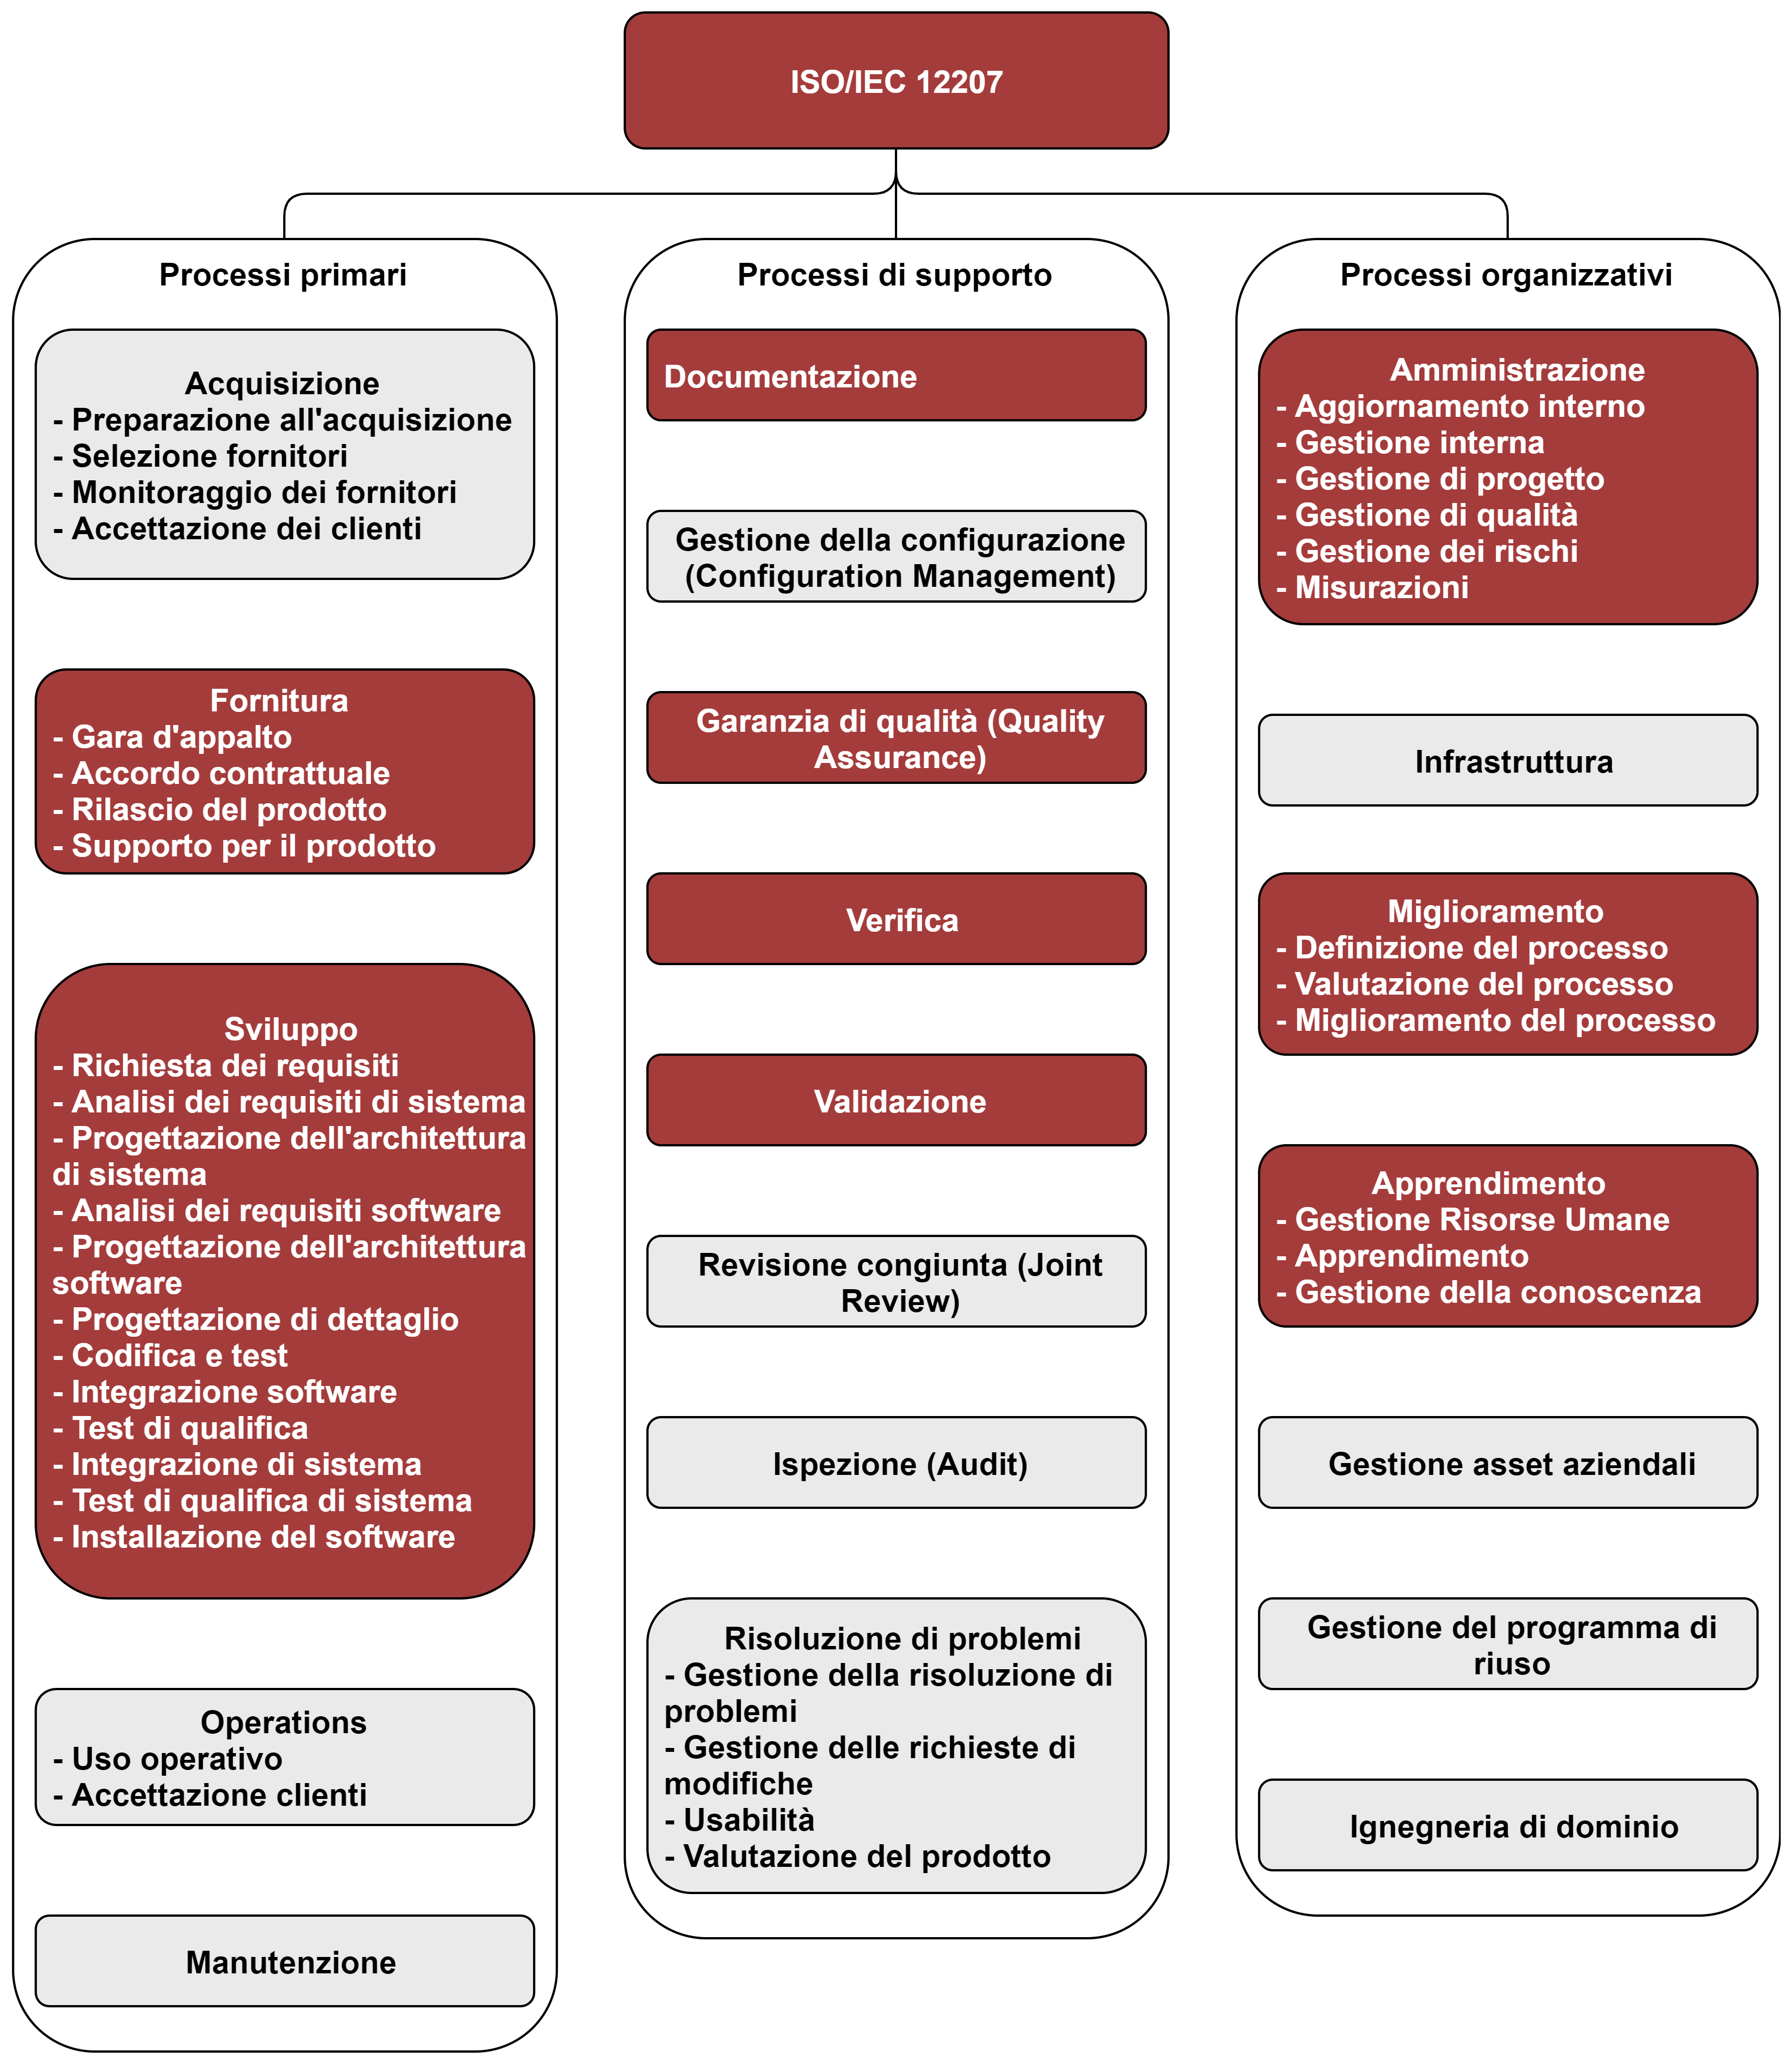
\includegraphics[scale=0.53]{Sezioni/Immagini/IsoIec12207.png}
    \caption{Schema dello standard ISO/IEC 12207. In rosso sono indicati i processi e le relative attività di interesse per il progetto.}
\end{figure}

\subsubsection{Processi primari}
Sono i \glo{processi} e le attività che fanno parte dello sviluppo del software e hanno lo scopo di soddisfare tutti i requisiti concordati con il cliente.

\paragraph{Sviluppo}\mbox{}\\ \\
Il \glo{processo} ha lo scopo di sviluppare un prodotto software, o un sistema basato sul software, che indirizzi le esigenze del cliente. \\
I risultati delle valutazioni dei \glo{processi} devono essere documentati.
\begin{itemize}
    \item \textbf{Analisi dei requisiti:} \\
    Lo sviluppatore deve valutare i requisiti software in base ai criteri elencati di seguito:
        \begin{itemize}
            \item Tracciabilità dei requisiti di sistema e progettazione del sistema;
            \item Coerenza esterna con i requisiti di sistema;
            \item Coerenza interna;
            \item \glo{Testabilità};
            \item Fattibilità della progettazione del software;
            \item Fattibilità di funzionamento e manutenzione.
        \end{itemize}
    \item \textbf{Pianificazione di dettaglio:} \\
    Lo sviluppatore deve sviluppare un progetto dettagliato per ciascun componente software. I componenti del software 
    devono essere perfezionati in livelli inferiori contenenti unità software che possono essere codificati, compilati 
    e testati. È necessario garantire che tutti i requisiti software siano assegnati dai componenti software 
    alle unità software.
    
    \item \textbf{Codifica:} \\
    Lo sviluppatore deve valutare il codice del software e i risultati dei test considerando i criteri elencati sotto:
    \begin{itemize}
        \item Tracciabilità ai requisiti e alla progettazione dell'articolo software;
        \item Coerenza esterna con i requisiti e il design dell'articolo software;
        \item Coerenza interna tra i requisiti dell'unità;
        \item Testare la copertura delle unità;
        \item Adeguatezza dei metodi e delle norme di codifica utilizzati;
        \item Fattibilità dell'integrazione e dei test del software;
        \item Fattibilità di funzionamento e manutenzione.   
    \end{itemize}
\end{itemize}

\subsubsection{Processi di supporto}
Sono i \glo{processi} e le attività che aiutano gli altri \glo{processi} nel raggiungimento del successo e nella qualità del progetto.

\paragraph{Documentazione}\mbox{}\\ \\
Il \glo{processo} di "Gestione della documentazione" garantisce lo sviluppo e la manutenzione delle informazioni prodotte e registrate relativamente al prodotto software. \\ \\
\textbf{Implementazione:} \\ 
Identifica i documenti da produrre durante il ciclo di vita del prodotto software;
deve essere sviluppato, documentato e implementato. La documentazione dovrà prevedere i seguenti punti: 
\begin{itemize}
    \item Titolo o nome;
    \item Scopo;
    \item Pubblico previsto;
    \item Procedure e responsabilità per input, sviluppo, revisione, modifica, approvazione, produzione, stoccaggio, distribuzione, manutenzione e gestione della configurazione;
    \item Programma per le versioni intermedie e finali.
\end{itemize}

\paragraph{Garanzia di qualità}\mbox{}\\ \\
Il \glo{processo} di "Assicurazione qualità" ha lo scopo di assicurare che tutti i prodotti di fase (work product) siano conformi con i piani e gli standard definiti.
\paragraph{Verifica}\mbox{}\\ \\
Il \glo{processo} di verifica ha lo scopo di confermare che ciascun work product o servizio realizzato da un \glo{processo} soddisfi i requisiti specificati. 
Il \glo{processo} di verifica deve essere integrato nei \glo{processi} di Sviluppo, Fornitura e Manutenzione. Se la verifica viene eseguita da terzi, questa viene definita come "\glo{Processo} di verifica indipendente".
\\
Il \glo{processo} deve essere verificato considerando i criteri elencati di seguito:
\begin{itemize}
    \item I requisiti di pianificazione del progetto sono adeguati e tempestivi;
    \item I \glo{processi} selezionati per il progetto sono adeguati, implementati, eseguiti come previsto, e conformi al contratto;
    \item Gli standard, le procedure e gli ambienti per i \glo{processi} del progetto sono adeguati;
    \item Il progetto è composto da personale qualificato capace di soddisfare le richieste del contratto.
\end{itemize}

\subsubsection{Processi organizzativi}
Sono i \glo{processi} e le attività che coprono gli aspetti organizzativi e di gestione delle risorse.

\paragraph{Gestione}\mbox{}\\ \\
Il \glo{processo} di gestione garantisce lo sviluppo e la manutenzione delle informazioni prodotte e registrate relativamente 
al prodotto software. L'amministratore prepara i piani per l'esecuzione del \glo{processo}.
I piani associati all'esecuzione del \glo{processo} devono contenere descrizioni: delle attività, dei compiti associati e
identificazioni dei prodotti software che verranno forniti. Questi piani devono rispettare i seguenti punti:
\begin{itemize}
    \item Programmi per il completamento tempestivo dei compiti;
    \item Risorse adeguate necessarie per eseguire i compiti;
    \item Assegnazione di compiti;
    \item Assegnazione di responsabilità;
    \item Quantificazione dei rischi associati ai compiti o al \glo{processo} stesso;
    \item Misure di controllo della qualità da applicare durante l'intero \glo{processo};
    \item Costi associati all'esecuzione del \glo{processo};
    \item Fornitura di ambiente e infrastruttura.
\end{itemize}

\subsection{ISO/IEC 9126}
Lo standard ISO/IEC 9126 si occupa di presentare le caratteristiche di qualità di un prodotto software e gli attributi che le compongono.

\begin{figure}[h]
    \centering
    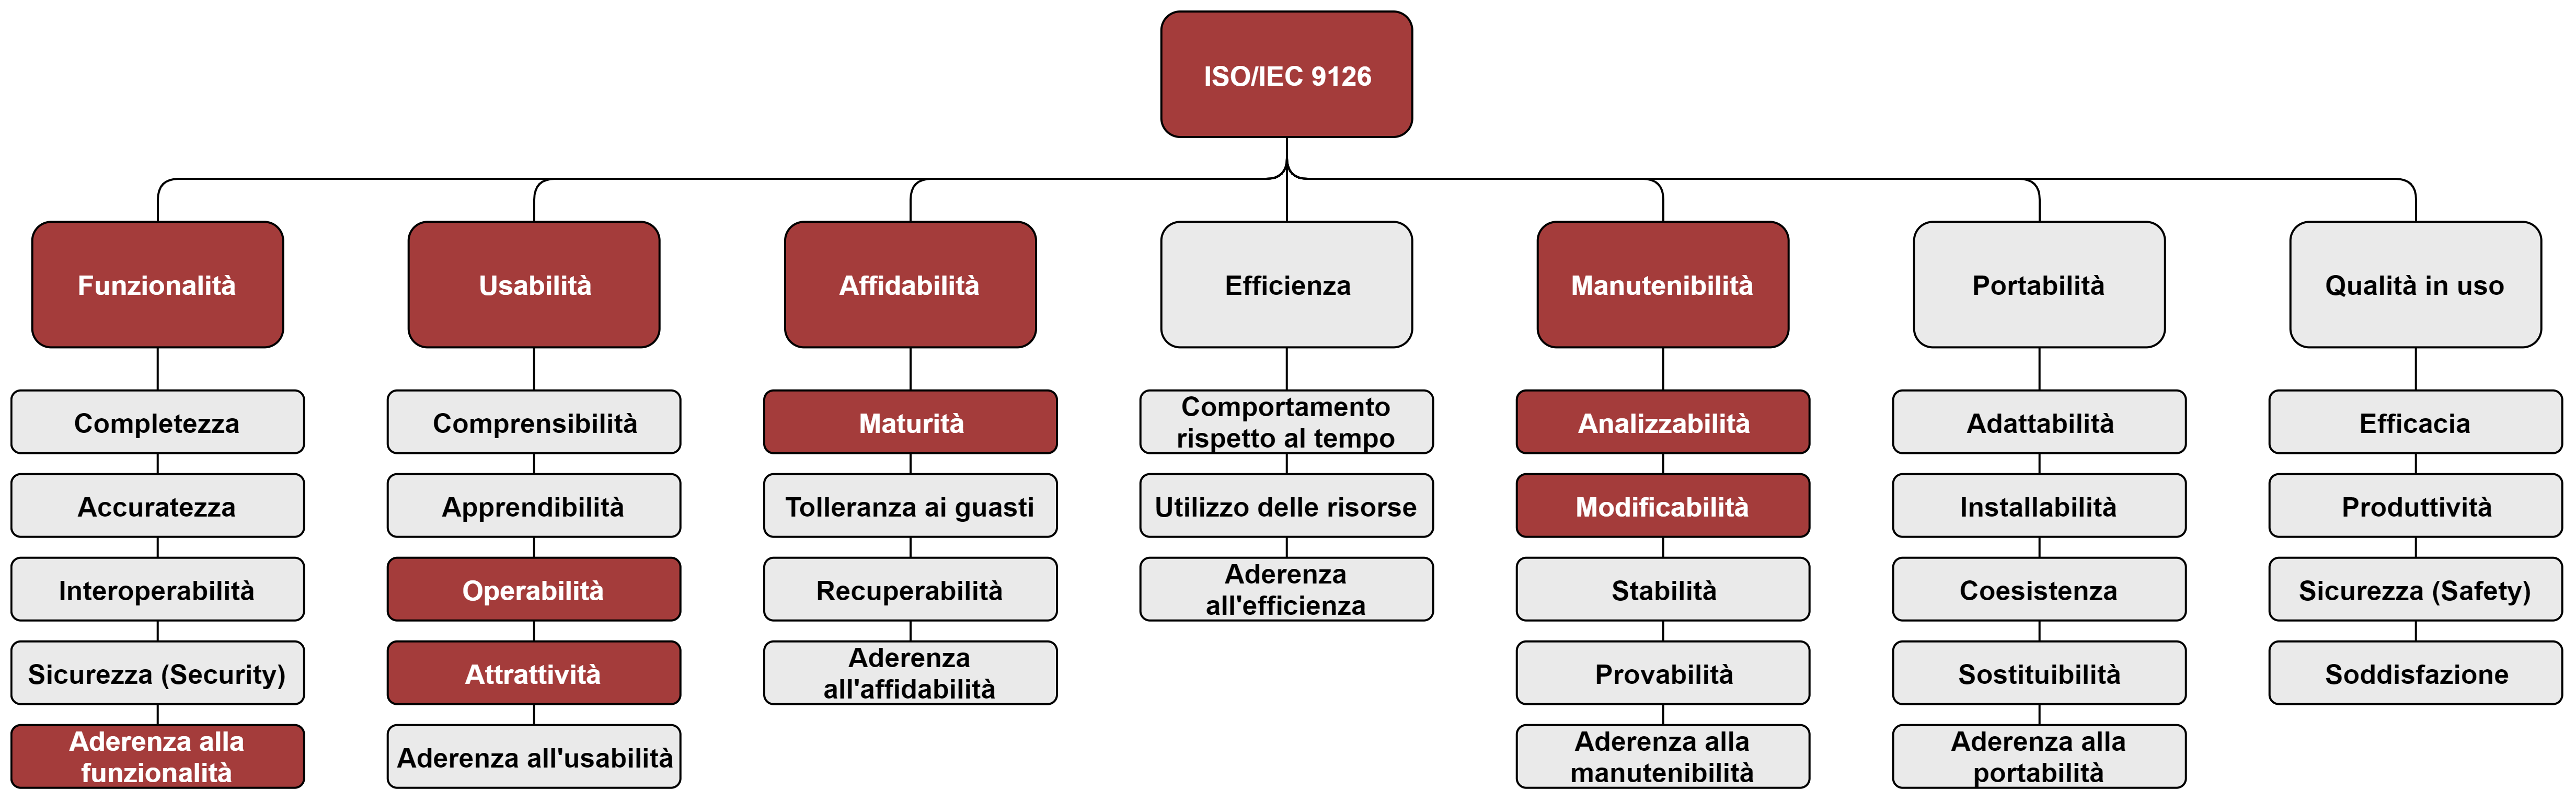
\includegraphics[scale=0.53]{Immagini/IsoIec9126.png}
    \caption{Schema dello standard ISO/IEC 9126. In rosso sono indicate le caratteristiche e attributi di interesse per il progetto.}
\end{figure}

\subsubsection{Metriche esterne}
Le metriche relative alla qualità "esterna" indirizzano le caratteristiche esteriori del software, cioè quelle rilevabili direttamente dagli utenti e dagli operatori.

\subsubsection{Metriche interne}
 Le metriche della qualità "interne" del software sono utilizzate durante la fase di sviluppo e permettono di valutare il comportamento del software dal punto di vista degli sviluppatori e di predire quello che sarà il punto di vista esterno degli utenti.

\subsubsection{Funzionalità}
Capacità del prodotto software di fornire funzioni adeguate al contesto di applicazione.
\begin{itemize}
\item \textbf{Adeguatezza}: Capacità di fornire un insieme di funzioni che permettano agli utenti del software di poter svolgere i loro compiti.
\item \textbf{Accuratezza}: Capacità di fornire i risultati attesi dall’utente con la precisione richiesta.
\item \textbf{Interoperabilità}: Capacità di interagire con uno o più sistemi specificati.
\item \textbf{Sicurezza (Security)}: Capacità di proteggere le informazioni e i dati dell’utente da persone non autorizzate ad accedervi.
\item \textbf{Aderenza alla funzionalità}: Capacità di aderire a standard, norme, convenzioni e regolamenti sulle funzionalità.
\end{itemize}

\subsubsection{Affidabilità}
Capacità del prodotto software di mantenere il livello di prestazione quando usato in condizioni specificate.
E’ limitata da errori nei requisiti, nella progettazione e nel codice del software.
\begin{itemize}
\item \textbf{Maturità}: Capacità di evitare che si verifichino errori.
\item \textbf{Tolleranza a guasti}: Capacità di mantenere il livello di prestazioni in caso di errori o violazione delle interfacce. Assieme alla \glo{Maturità}, descrivono l’attributo \glo{Disponibilità}, non specificato in quanto formato da questi due.
\item \textbf{Recuperabilità}: Capacità di ripristinare il livello di prestazioni e i dati in caso di errori e malfunzionamenti.
\item \textbf{Aderenza all’affidabilità}: Capacità di aderire a standard, norme, convenzioni e regolamenti sull’affidabilità.
\end{itemize}

\subsubsection{Usabilità}
Capacità del prodotto software di essere comprensibile, di poter essere studiato.
\begin{itemize}
\item \textbf{Comprensibilità}: Capacità di permettere all’utente di capire le funzionalità e come usarle con successo;
\item \textbf{Apprendibilità}: Capacità di permettere all’utente di imparare l’applicazione;
\item \textbf{Operabilità}: Capacità di permettere all’utente di usare il software e controllarlo;
\item \textbf{Attrattività}: Capacità di risultare attraente (ossia possedere una interfaccia utente accattivante);
\item \textbf{Aderenza all’usabilità}: Capacità di aderire a standard, norme, convenzioni e regolamenti sull’usabilità.
\end{itemize}

\subsubsection{Efficienza}
Capacità del prodotto software di realizzare le funzioni richieste nel minor tempo possibile.
\begin{itemize}
\item \textbf{Comportamento rispetto al tempo}: Capacità di fornire in tempi adeguati risposte per l’utente;
\item \textbf{Utilizzo risorse}: Capacità di utilizzare un appropriato numero e tipo di risorse, eseguendo le funzionalità previste;
\item \textbf{Aderenza all’efficienza}: Capacità di aderire a standard, norme, convenzioni e regolamenti sull’efficienza.
\end{itemize}

\subsubsection{Manutenibilità}
Capacità del prodotto software di essere modificato.
\begin{itemize}
\item \textbf{Analizzabilità}: Capacità di poter diagnosticare errori e individuare malfunzionamenti;
\item \textbf{Modificabilità}: Capacità di consentire lo sviluppo di modifiche al software originale;
\item \textbf{Stabilità}: Capacità di evitare effetti non desiderati;
\item \textbf{Provabilità}: Capacità di consentire la verifica delle funzionalità del prodotto software;
\item \textbf{Aderenza alla manutenibilità}: Vpacità di aderire a standard, norme, convenzioni e regolamenti sulla manutenibilità.
\end{itemize}

\subsubsection{Portabilità}
Capacità di essere trasportato da un ambiente ad un altro.
\begin{itemize}
\item \textbf{Adattabilità}: Verrà descritta se ce ne sarà il bisogno;
\item \textbf{Installabilità}: Verrà descritta se ce ne sarà il bisogno;
\item \textbf{Coesistenza}: Verrà descritta se ce ne sarà il bisogno;
\item \textbf{Aderenza alla portabilità}: Verrà descritta se ce ne sarà il bisogno.
\end{itemize}

\subsubsection{Qualità in uso}
\begin{itemize}
\item \textbf{Efficacia}: Capacità per l’utente del prodotto software di raggiungere obiettivi specifici con \glo{accuratezza} e \glo{completezza};
\item \textbf{Produttività}: Capacità di permettere all’utente di impegnare un numero definito di risorse, in relazione all’efficienza raggiunta. Queste risorse possono essere tempo, materiali e costi;
\item \textbf{Sicurezza fisica (Safety)}: Capacità di raggiungere un livello accettabile di rischio per dati, business e persone. I rischi sono tipicamente correlati a difetti in progettazione o analisi o codifica;
\item \textbf{Soddisfazione}: Capacità di soddisfare gli utenti in uno specifico contesto.
\end{itemize}

\subsubsection{Piano di Qualifica}
Nel documento \PdQ{} il gruppo \Gruppo{} illustra come intende gestire la qualità di processo e di qualità di prodotto, elenca le varie metriche definite per aderire alle definizioni degli standard e i test per verificare la corretta soddisfazione dei requisiti del prodotto software.\newline
La qualità di processo e la qualità di prodotto sono due aspetti chiaramente coordinati, ma vengono gestiti separatamente.
Le sezioni principali del documento sono le seguenti:
\begin{itemize}
    \item \textbf{Qualità di processo:} Sezione dove vengono elencate le metriche inerenti ai \glo{processi};
    \item \textbf{Qualità di prodotto:} Sezione dove vengono elencate le metriche inerenti al prodotto;
    \item \textbf{Strategia di testing:} Sezione dove viene elencato il piano di testing delle componenti e del sistema software nel suo complesso;
    \item \textbf{Standard di qualità adottati:} Sezione dove vengono spiegati gli standard adottati.
\end{itemize}

\subsubsection{Metriche di qualità}
\paragraph{Codici metriche}\mbox{}
Ogni metrica di \glo{processo} ha un codice univoco ed è strutturato in questo formato:
\begin{center}
    M[Destinazione][Numero progressivo]
\end{center}
con:
\begin{itemize}  
    \item \textbf{[Destinazione]}:
    \begin{itemize}
        \item \textbf{PC}: Se la metrica fa riferimento al \glo{processo};
        \item \textbf{PD}: Se la metrica fa riferimento al prodotto.
    \end{itemize}
    \item \textbf{[Numero progressivo]}: Il numero della metrica in relazione alla sua destinazione, progressivo perché diverso per ogni metrica e in serie. Il conteggio parte da 1.
\end{itemize}

\paragraph{Struttura descrittiva metriche}
La seguente è una struttura ad elenco che descrive una metrica di processo o di prodotto. \\
I punti dell'elenco racchiusi fra parentesi quadre indicano che tale punto è opzionale e va inserito solo se necessario.\\
Inoltre, \textbf{Processo di riferimento} deve essere presente solo nelle metriche della qualità di processo, mentre \textbf{Attributo di riferimento} solo per la qualità di prodotto.
elencata in una lista, mentre il nome della metrica rappresenta il titolo di questo elenco ed è visibile nell'indice del documento. La struttura è la seguente:
\begin{itemize}
    \item \textbf{Codice}: Codice univoco;
    \item \textbf{Descrizione}: Breve descrizione della metrica e del contesto applicativo;
    \item \textbf{Processo di riferimento}: Viene indicata in quale \glo{processo} viene applicata tale metrica (riferendosi allo standard);
    \item \textbf{Attributo di riferimento}: Viene indicato in quale attributo della caratteristica di prodotto viene applicata tale metrica (riferendosi allo standard);
    \item \textbf{Sigla}: nome della metrica sotto forma di acronimo, utilizzato principalmente nelle formule matematiche e nei range di accettazione;
    \item \textbf{[Formula:} formula matematica per poter calcolare il valore della metrica];
    \item \textbf{Range di valori che può assumere}: sezione in cui sono descritti i range di accettazione per i valori delle metriche.
    \begin{itemize}
        \item \textbf{Accettabile}: range in cui i valori della metrica possono essere ritenuti accettabili per garantire la qualità;
        \item \textbf{Ottimale}: range in cui i valori della metrica possono essere ritenuti ottimali per garantire la qualità.
    \end{itemize}
\end{itemize}

\paragraph{Metriche di processo}
Per monitorare l'aderenza ai processi dallo standard ISO/IEC 12207 istanziati, vengono utilizzate delle metriche. Il Responsabile, grazie ai valori ricavati dalle metriche, è facilitato nel valutare il \glo{processo} e di effettuare, se necessario, modifiche alla pianificazione.

\paragraph{Metriche di prodotto}
Il modello di qualità del software descritto dallo standard ISO/IEC 9126 definisce le caratteristiche e gli attributi del prodotto software, ciascuna misurabile da metriche interne (che richiedono la disponibilità del codice sorgente - white box) o esterne (che richiedono il prodotto software in esecuzione - black box).
Una volta specificati i requisiti di qualità del prodotto software, si identificano le caratteristiche e attributi di qualità che più contribuiscono a verificare l'aderenza allo standard e ai requisiti.
Il gruppo \Gruppo{} si è impegnato a scegliere le metriche interne che maggiormente influenzano (in positivo) le caratteristiche esterne del prodotto finale, in modo che esse possano predire quanto più possibile la qualità del risultato finale. 

\paragraph{Tabella riassuntiva metriche}
Per riassumere tutte le metriche e le loro caratteristiche descritte all'interno del \PdQ{}, alla fine della sezione in cui vengono illustrate vi sono delle tabelle riassuntive che hanno questa struttura:
{
\rowcolors{2}{grigetto}{white}
\renewcommand{\arraystretch}{1.5}
\begin{longtable}{ c C{4cm} c C{3.5cm} C{3.5cm}}
\caption{Tabella metriche dei processi/prodotti}\\
\rowcolor{darkblue}
\textcolor{white}{\textbf{Metrica}} & \textcolor{white}{\textbf{Nome}} & \textcolor{white}{\textbf{Sigla}} & \textcolor{white}{\textbf{Range Accettabile}} & \textcolor{white}{\textbf{Range Ottimale}}\\
Codice & Nome della metrica & Sigla & Range Accettabile & Range Ottimale \\
\end{longtable}
}

\subsubsection{Lista delle metriche di processo}
\paragraph{Processi di supporto}

\subparagraph{Verifica}
\subsubparagraph{Metrica - Code coverage}
\begin{itemize}
	\item \textbf{Codice:} MPC7
	\item \textbf{Descrizione:} È la percentuale di copertura del codice attraversato dai test rispetto al totale del codice di base. Per dare una misurazione in termini di grandezza si adoperano le linee di codice come riferimento;
	\item \textbf{Processo di riferimento:} \glo{Processi} di verifica;
	\item \textbf{Sigla:} $CC$
	\item \textbf{Formula:} $$CC = \frac{|linee \; di \; codice \; percorse \; dai  \; test|}{|linee \; di \; codice \; totali|} \; \cdot \; 100$$
	\item \textbf{Strumenti utilizzati:} \glo{SonarQube}.
\end{itemize}
   \paragraph{Processi organizzativi}

\subparagraph{Pianificazione}

\subsubparagraph{Metrica - Actual Cost of Work Performed}
    \begin{itemize}
        \item \textbf{Codice:} MPC8
        \item \textbf{Descrizione:} Denaro speso fino al momento del calcolo;
        \item \textbf{Processo di riferimento:} Gestione;
        \item \textbf{Sigla:} $ACWP$
        \item \textbf{Formula:} $$ACWP = {Sommatoria\; delle\; ore\; lavorative\; moltiplicate\; con\; il\; corrispondente\; costo\; orario}$$
        \item \textbf{Strumenti utilizzati:} Fogli Google.
    \end{itemize}

\subsubparagraph{Metrica - Budgeted Cost of Work Scheduled}
\begin{itemize}
	\item \textbf{Codice:} MPC9
    \item \textbf{Descrizione:} Costo pianificato per realizzare le attività di progetto pianificate fino al momento del calcolo.
    Per attività di progetto pianificate si intendono il numero di requisiti che devono soddisfatti dal prodotto software;
	\item \textbf{Processo di riferimento:} Gestione;
	\item \textbf{Sigla:} $BCWS$
	\item \textbf{Formula:} $$BCWS = {B_{tot} * \% \;di\; lavoro\; pianificato}$$
	con:
	\begin{itemize}
		\item $B_{tot}$ = Budget totale.
	\end{itemize}
	\item \textbf{Strumenti utilizzati:} Fogli Google.
\end{itemize}

\subsubparagraph{Metrica - Budgeted Cost of Work Performed}
\begin{itemize}
	\item \textbf{Codice:} MPC10
	\item \textbf{Descrizione:} Il costo del lavoro fatto fino al momento del calcolo, ovvero la variazione del numero di requisiti soddisfatti nel periodo in cui la metrica viene calcolata;
	\item \textbf{Processo di riferimento:} Gestione;
	\item \textbf{Sigla:} $BCWP$
	\item \textbf{Formula:} $$BCWP = {B_{tot} * \% \;di\; lavoro\; svolto}$$
	con:
	\begin{itemize}
		\item $B_{tot}$ = Budget totale.
	\end{itemize}
	\item \textbf{Strumenti utilizzati:} Fogli Google.
\end{itemize}

    \subsubparagraph{Metrica - Schedule variance}
    \begin{itemize}
        \item \textbf{Codice:} MPC11
        \item \textbf{Descrizione:} È il valore che indica se si è in linea ($=0$), in anticipo ($>0$) oppure in ritardo ($<0$) rispetto alla schedulazione delle attività di progetto pianificate nella \glo{baseline};
        \item \textbf{Processo di riferimento:} Gestione;
        \item \textbf{Sigla:} $SV$
        \item \textbf{Formula:} $$SV = {BCWP \; - \; BCWS}$$
        con:
        \begin{itemize}
            \item $BCWP$ = Budgeted Cost of Work Performed (valore delle attività eseguite nella data corrente);
            \item $BCWS$ = Budgeted Cost of Work Scheduled (costo pianificato per la realizzazione delle attività di progetto alla data corrente);
        \end{itemize}
    \item \textbf{Strumenti utilizzati:} Fogli Google.
    \end{itemize}

    \subsubparagraph{Metrica - Budget variance}
        \begin{itemize}
            \item \textbf{Codice:} MPC12
            \item \textbf{Descrizione:} È il valore che indica se alla data corrente si è speso di più ($>0$) o di meno ($<0$) rispetto a quanto pianificato dal budget totale $B_{tot}$;
            \item \textbf{Processo di riferimento:} Gestione;
            \item \textbf{Sigla:} $BV$
            \item \textbf{Formula:} $$BV = {BCWS \; - \; ACWP}$$
            con:
            \begin{itemize}
                \item $BCWS$ = Budgeted Cost of Work Scheduled (costo pianificato per la realizzazione delle attività di progetto alla data corrente);
                \item $ACWP$ = Actual Cost of Work Performed (costo effettivamente sostenuto alla data corrente);
                \item $B_{tot}$ = Budget totale.
            \end{itemize}
        \item \textbf{Strumenti utilizzati:} Fogli Google.
        \end{itemize}
\newpage
\subsubsection{Lista delle metriche di prodotto}
\paragraph{Metriche interne}
Le metriche della qualità "interne" del software sono utilizzate durante la fase di sviluppo e permettono di valutare il comportamento del software dal punto di vista degli sviluppatori e di predire quello che sarà il punto di vista esterno degli utenti.

\subparagraph{Usabilità}
Capacità del prodotto software di essere comprensibile, di poter essere usato e compreso facilmente, in ogni sua parte, da qualsiasi utente che lo voglia usare.\\

\subsubparagraph{Metrica - Attrattività della User Interface (UI)} 
\begin{itemize}
    \item \textbf{Codice:} MPD1
    \item \textbf{Descrizione:} Misurare quanto attrattive risultino le interfacce agli utenti dal punto di vista grafico.
    Gli utenti dovranno poi compilare un questionario in base all'esperienza che hanno fatto;
    Il valore medio di tale valutazione è ritenuto valido se almeno tre utenti hanno compilato il questionario. 
    Viene utilizzata una scala a quattro valori: Molto attrattivo, Attrattivo, Poco attrattivo, Non Attrattivo;
    \item \textbf{Attributo di riferimento:} \glo{Attrattività};
    \item \textbf{Sigla:} $AUI$
    \item \textbf{Formula:}$$AUI = V(q) $$
    con:
        \begin{itemize}
        \item $V$ = Valore medio dei risultati;
        \item $q$ = Questionario compilato;
        \end{itemize}
    \item \textbf{Strumenti utilizzati:} Moduli Google.
\end{itemize}

\subparagraph{Manutenibilità}
Capacità di predire il livello di impegno richiesto per modificare il prodotto software dal punto di vista degli sviluppatori.           
\subsubparagraph{Metrica - Complessità Ciclomatica del Software} 
    \begin{itemize}
    \item \textbf{Codice:} MPD2
    \item \textbf{Descrizione:} Misurare la complessità ciclomatica dei singoli moduli sviluppati;
    \item \textbf{Attributo di riferimento:} \glo{Modificabilità};
    \item \textbf{Sigla:} $CCS$
    \item \textbf{Formula:} $$CCS = e - n + p$$
    con:
    \begin{itemize}
        \item $G$ = grafo del modulo;
        \item $e$ = numero di congiunzioni tra statement (corrispondenti agli archi di un grafo);
        \item $n$ = numero di statement (nodi presenti nel grafo);
        \item $p$ = numero delle componenti connesse da ogni nodo (per esecuzione sequenziale: p=2, essendovi un predecessore e un successore);
    \end{itemize}
    \item \textbf{Strumenti utilizzati:} Non ancora definito.
\end{itemize}

\subsubparagraph{Metrica - Unità Documentate} 
\begin{itemize}
    \item \textbf{Codice:} MPD3
    \item \textbf{Descrizione:} Misurare in percentuale il numero di unità di codice con documentazione tecnica;
    \item \textbf{Attributo di riferimento:} \glo{Modificabilità};
    \item \textbf{Sigla:} $UD$
    \item \textbf{Formula:} $$UD = \frac{|unit\grave{a} \; di \; codice \; con \; documentazione \; tecnica|}{|unit\grave{a} \; di \; codice|} \cdot 100$$
    \item \textbf{Strumenti utilizzati:} Non ancora definito.
\end{itemize}
              
       
\paragraph{Metriche esterne}
Le metriche relative alla qualità "esterna" indirizzano le caratteristiche esteriori del software, cioè quelle rilevabili direttamente dagli utenti e dagli operatori.

\subparagraph{Affidabilità}
Capacità del prodotto software di dimostrare un adeguato livello di affidabilità quando opererà nel sistema in cui è previsto debba operare.
  
\subsubparagraph{Metrica - Presenza di code smell} 
\begin{itemize}
    \item \textbf{Codice:} MPD4
    \item \textbf{Descrizione:} Misurare il numero di \glo{code smell} presenti all'interno del codice del prodotto;
    \item \textbf{Attributo di riferimento:} \glo{Manutenibilità};
    \item \textbf{Sigla:} $CS$
    \item \textbf{Formula:} $$CS = {numero \; di \; code \; smell \; rilevati}$$
    \item \textbf{Strumenti utilizzati:} \glo{SonarQube}.
\end{itemize}

\subsubparagraph{Metrica - Presenza di vulnerabilità} 
\begin{itemize}
    \item \textbf{Codice:} MPD5
    \item \textbf{Descrizione:} Misurare il numero di \glo{vulnerabilità} presenti all'interno del codice del prodotto;
    \item \textbf{Attributo di riferimento:} \glo{Sicurezza};
    \item \textbf{Sigla:} $VLN$
    \item \textbf{Formula:} $$VLN = {numero \; di \; vulnerabilit\grave{a} \; rilevate}$$
    \item \textbf{Strumenti utilizzati:} \glo{SonarQube}.
\end{itemize}

\subsubparagraph{Metrica - Presenza di bug} 
\begin{itemize}
    \item \textbf{Codice:} MPD6
    \item \textbf{Descrizione:} Misurare il numero di \glo{bug} presenti all'interno del codice del prodotto;
    \item \textbf{Attributo di riferimento:} \glo{Operabilità};
    \item \textbf{Sigla:} $BUG$
    \item \textbf{Formula:} $$BUG = {numero \; di \; bug \; rilevati}$$
    \item \textbf{Strumenti utilizzati:} \glo{SonarQube}.
\end{itemize}

\subsubparagraph{Metrica - Maturità dei Test} 
\begin{itemize}
    \item \textbf{Codice:} MPD7
    \item \textbf{Descrizione:} Misurare la percentuale di casi di test eseguiti con successo rispetto al numero totale previsto per garantire piena copertura dei requisiti sia funzionali che qualitativi(usabilità, affidabilità, efficienza);
    \item \textbf{Attributo di riferimento:} \glo{Maturità};
    \item \textbf{Sigla:} $MT$
    \item \textbf{Formula:} $$MT = \frac{|casi \; di \; test \; eseguiti \; con \; successo|}{|casi \; di \; test \; previsti|} \cdot 100$$
    \item \textbf{Strumenti utilizzati:} Non ancora definito.
\end{itemize}
       
\subparagraph{Usabilità}
Capacità del prodotto software di essere facilmente comprensibile, apprendibile ed operabile per ogni utente intenzionato a usarlo.

\subsubparagraph{Metrica - Profondità Strutturale dell'Interfaccia}
\begin{itemize}
    \item \textbf{Codice:} MPD8
    \item \textbf{Descrizione:} È sconsigliato per le interfacce utente l'utilizzo di una struttura troppo profonda per questioni di usabilità. L'utente non deve fare troppi passaggi per raggiungere la funzionalità desiderata;
    \item \textbf{Attributo di riferimento:} \glo{Operabilità};
    \item \textbf{Sigla:} $PSI$
    \item \textbf{Strumenti utilizzati:} Controllo manuale.
\end{itemize}
\newpage
%scritto da \PF{} e\AT{}
\subsection{Verifica}
\subsubsection{Scopo}
Il processo di verifica si pone l’obiettivo di perseguire la realizzazione di un prodotto corretto e conforme alle aspettative degli \glo{stakeholder}, in particolar modo assicurandosi che l'esecuzione delle attività dei processi non introduca errori.
Deve essere svolto durante ogni \glo{fase} del ciclo di vita del software.
\subsubsection{Aspettative}
Per un corretto svolgimento del processo di verifica si devo rispettare i seguenti punti:
\begin{itemize} 
    \item individuare le tecniche di verifica;
    \item individuare gli strumenti di verifica;
    \item individuare e correggere i difetti applicando gli strumenti;
    \item provare che il sistema soddisfi i requisiti.
\end{itemize}
\subsubsection{Descrizione}
Il processo di verifica prende in input ciò che è stato prodotto sia nella documentazione sia nel codice e lo restituisce in uno stato conforme alle aspettative tramite a processi di test. Ad termine del corretto svolgimento del processo di verifica sussegue il processo di validazione.
\subsubsection{Attività}
Per eseguire il processo di verifica vengono svolte le seguenti attività:
\begin{itemize} 
    \item \textbf{Analisi statica};
    \item \textbf{Analisi dinamica}.
\end{itemize}
\paragraph{Implementazione del processo}
\subparagraph*{Analisi statica} 
L'analisi statica è un'attività di verifica da effettuare fin da subito sulla documentazione prodotta e, non appena disponibile, sul codice sorgente, poiché non richiede alcuna esecuzione.
Essa si accerta che ciò che il gruppo ha prodotto sia conforme alle regole indicate nel \PdQ{}, che non ci siano errori e difetti, e che siano invece presenti le proprietà desiderate.
Per effettuare l’attività di analisi statica vengono impiegati due possibili metodi: \textbf{walkthrough} e \textbf{inspection}.

\subparagraph*{Walkthrough} 
Il walkthrough è un metodo di verifica effettuato da tutti i membri del gruppo, e non solo dai verificatori, il cui obiettivo è rilevare la presenza di difetti o anomalie senza aver effettuato alcuna assunzione.
Per il codice devono essere verificate tutte le possibili esecuzioni, mentre per i documenti si devono esaminare tutte le parti che li compongono.
Questo metodo è utile da applicare nel periodo iniziale del progetto (antecedente alla RR), dato che non è ancora ben chiara la forma del prodotto che si sta realizzando.
Inoltre, non tutti membri del gruppo hanno ampie conoscenze in tema di verifica, a maggior ragione su questo progetto. Una volta che il prodotto in realizzazione viene considerato acquisito da tutto il gruppo, il walkthrough può venire sostituito con altri metodi meno onerosi e più mirati.
\subparagraph*{Inspection}
L'inspection è un metodo di verifica effettuato dai verificatori, il cui obiettivo è effettuare verifiche mirate sugli aspetti critici del prodotto al fine di rilevare la presenza di difetti e/o anomalie.
I verificatori, una volta acquisita una più ampia conoscenza sul prodotto da verificare, costruiscono e utilizzano una lista all’interno della quale vi sono gli aspetti critici da andare a verificare e dove verificarli.

\subparagraph*{Analisi dinamica} 
L'analisi dinamica è un'attività di verifica che viene eseguita esclusivamente sul prodotto software (e non sulla documentazione), in quanto ne richiede l'esecuzione per essere effettuata.
Viene applicata sul prodotto software attraverso i test, con l’obiettivo di individuarne difetti e/o anomalie.

\subparagraph*{Test} 
I test sono necessari per poter svolgere l'analisi dinamica del prodotto software.
I test devono essere automatici e ripetibili:
\begin{itemize}
\item \textbf{Automatici}: Per automatici si intende la necessità di disporre di un'automazione (per esempio un comando da \glo{CLI}) che permetta a tutti i membri del gruppo di invocare ed eseguire tutti (o in parte) i test.
I test devono poter essere eseguiti semplicemente e non devono richiedere alcuna interazione umana.
Devono essere rapidi nell’esecuzione e in grado di riconoscere e notificare la presenza di errori;
\item \textbf{Ripetibili}: Per ripetibili si intende che ogni invocazione di test deve produrre sempre lo stesso risultato dato uno stesso insieme di dati in input.
Per garantire questa caratteristica serve che ci sia determinismo, che è garantito se:
\begin{itemize}
    \item Fra un'esecuzione di un test e l'altra non varia l'ambiente d'esecuzione (ovvero non cambia l'hardware e nemmeno il software);
    \item Non cambia lo stato iniziale del sistema.
\end{itemize}
\end{itemize}
Per ogni test, verrà costruita una tabella dove verranno riportato il loro stato di esecuzione:
\begin{itemize}
	\item \textbf{NS}: Il test non è stato superato;
	\item \textbf{S}: Il test è stato superato;
	\item \textbf{NI}: Il test non è stato implementato;
	\item \textbf{I}: Il test è stato implementato.
\end{itemize}

Ci sono diverse tipologie di test del software, ognuna delle quali ha un diverso oggetto di verifica e scopo.

\subparagraph*{Test di unità} 
I test di unità sono del codice, prodotti dal programmatore, che verificano il corretto comportamento di una singola unità del programma.
Per unità si intende una funzionalità atomica che può essere verificata in modo isolato, in modo da assicurare che il risultato del test non sia influenzato dal comportamento di altre unità. In questo senso un'unità può essere un metodo, una classe o addirittura un package.
È definito modulo una frazione dell'unità.
Tipicamente l'autore di un test d'unità è il programmatore che ha codificato l'unità verificata dal test stesso.
L'obiettivo è verificare l’assenza di errori e documentare il comportamento dell’unità prodotta.
Per i test di unità vengono introdotti i seguenti concetti:
\begin{itemize}
    \item \textbf{driver}: Componente attiva che pilota i test e permette l'esecuzione automatizzata;
    \item \textbf{stub}: Componente passiva che simula il comportamento di un modulo dell'unità (si vuole verificare l'unità e non l'integrazione fra questa e il modulo);
    \item \textbf{logger}: Componente non intrusivo che registra gli esiti dell'esecuzione dei test.
\end{itemize}
Ogni test di unità è identificato da un codice univoco, così formato:
\begin{center}
	\item \textbf{TU[Destinazione][Numero progressivo]}
\end{center}
con:
\begin{itemize}
	\item \textbf{[Destinazione]}:
	\begin{itemize}
		\item \textbf{A}: Test di sistema che fa riferimento all'applicazione;
		\item \textbf{W}: Test di sistema che fa riferimento alla web-app;
		\item \textbf{B}: Test di sistema che fa riferimento al server.
	\end{itemize}
	\item \textbf{[Numero progressivo]}: Il numero del test di unità in relazione alla sua destinazione, progressivo perché diverso per ogni test e in serie. Il conteggio parte da 1.
\end{itemize}

\subparagraph*{Test d’integrazione} 
Servono per verificare incrementalmente il corretto funzionamento delle componenti del sistema.
Una volta che le unità sono verificate e passano con successo i relativi test, è possibile verificare il loro comportamento quando eseguite assieme.
Ogni test d’integrazione è identificato da un codice univoco, così formato:
\begin{center}
	\item \textbf{TI[Destinazione][Numero progressivo]}
\end{center}
con:
\begin{itemize}
	\item \textbf{[Destinazione]}:
	\begin{itemize}
		\item \textbf{A}: Test di sistema che fa riferimento all'applicazione;
		\item \textbf{W}: Test di sistema che fa riferimento alla web-app;
		\item \textbf{B}: Test di sistema che fa riferimento al server.
	\end{itemize}
	\item \textbf{[Numero progressivo]}: Il numero del test d’integrazione in relazione alla sua destinazione, progressivo perché diverso per ogni test e in serie. Il conteggio parte da 1.
\end{itemize}

\subparagraph*{Test di sistema} 
I test di sistema verificano il comportamento dell’intero sistema.
Si è quindi nella fase in cui tutte le componenti del sistema sono state integrate (i test di integrazione e di unità passano con successo) e si può verificare il loro comportamento all’interno del sistema in cui il prodotto dovrà essere installato o reso disponibile.
L'obiettivo è verificare che siano rispettati i requisiti definiti con il committente.
Quando questi test vengono svolti con la presenza del committente vengono definiti \textbf{test di accettazione} o \textbf{collaudo}. Se superati, permettono di procedere con il rilascio del prodotto software.
Ogni test di sistema è identificato da un codice univoco, così formato:
\begin{center}
    	\item \textbf{TS[Destinazione][Numero progressivo]}
\end{center}
con:
\begin{itemize}
    \item \textbf{[Destinazione]}:
    \begin{itemize}
        \item \textbf{A}: Test di sistema che fa riferimento all'applicazione;
        \item \textbf{S}: Test di sistema che fa riferimento al server.
    \end{itemize}
    \item \textbf{[Numero progressivo]}: Il numero del test di sistema in relazione alla sua destinazione, progressivo perché diverso per ogni test e in serie. Il conteggio parte da 1.
\end{itemize}

\subparagraph*{Test di regressione}
I test di regressione hanno come obiettivo di verificare l'assenza di regressioni (ovvero malfunzionamenti o comportamenti imprevisti) nel caso in cui si introduca una modifica su una componente dalla quale ne dipendono altre.
L'obiettivo di questi test è verificare che le componenti continuino a funzionare correttamente senza anomalie, ossia verificare che una modifica non pregiudichi le funzionalità già verificate con i test effettuati in precedenza.
Non è necessario identificare nuovi test, è sufficiente accertarsi che quelli presenti restituiscano i valori attesi.


\subsubsection{Metriche}

\paragraph{Code coverage}
\begin{itemize}
	\item \textbf{Codice:} MPC7
	\item \textbf{Descrizione:} È la percentuale di copertura del codice attraversato dai test rispetto al totale del codice di base. Per dare una misurazione in termini di grandezza si adoperano le linee di codice come riferimento;
	\item \textbf{Processo di riferimento:} \glo{Processi} di verifica;
	\item \textbf{Sigla:} $CC$
	\item \textbf{Formula:} $$CC = \frac{|linee \; di \; codice \; percorse \; dai  \; test|}{|linee \; di \; codice \; totali|} \; \cdot \; 100$$
	\item \textbf{Strumenti utilizzati:} Coveralls.
\end{itemize}

\paragraph{Documentazione - Branch Coverage}
\begin{itemize}
    \item \textbf{Codice:} MPC14
    \item \textbf{Descrizione:} Percentuale di rami condizionali coperti da test;
    \item \textbf{Processo di riferimento:} Verifica;
    \item \textbf{Sigla:} $BC$
    \item \textbf{Formula:} $$BC = \frac{|rami \; condizionali \; coperti \; da \; test|}{|rami \; condizionali \; totali|} \; \cdot \; 100$$;
    \item \textbf{Strumenti utilizzati:} Coveralls.
\end{itemize}

\paragraph{Documentazione - Statement Coverage}
\begin{itemize}
    \item \textbf{Codice:} MPC15
    \item \textbf{Descrizione:} Percentuale di istruzioni coperte da test;
    \item \textbf{Processo di riferimento:} Verifica;
    \item \textbf{Sigla:} $SC$
    \item \textbf{Formula:} $$SC = \frac{|istruzioni \; coperte \; da \; test|}{|istruzioni \; totali|} \; \cdot \; 100$$;
    \item \textbf{Strumenti utilizzati:} Coveralls.
\end{itemize}

\paragraph{Presenza di Code Smell} 
\begin{itemize}
    \item \textbf{Codice:} MPD4
    \item \textbf{Descrizione:} Misurare il numero di \glo{code smell} presenti all'interno del codice del prodotto;
    \item \textbf{Attributo di riferimento:} \glo{Manutenibilità};
    \item \textbf{Sigla:} $CS$
    \item \textbf{Formula:} $$CS = {numero \; di \; code \; smell \; rilevati}$$
    \item \textbf{Strumenti utilizzati:} \glo{SonarQube}.
\end{itemize}

\paragraph{Presenza di Vulnerabilità} 
\begin{itemize}
    \item \textbf{Codice:} MPD5
    \item \textbf{Descrizione:} Misurare il numero di \glo{vulnerabilità} presenti all'interno del codice del prodotto;
    \item \textbf{Attributo di riferimento:} \glo{Sicurezza};
    \item \textbf{Sigla:} $VLN$
    \item \textbf{Formula:} $$VLN = {numero \; di \; vulnerabilit\grave{a} \; rilevate}$$
    \item \textbf{Strumenti utilizzati:} \glo{SonarQube}.
\end{itemize}

\paragraph{Presenza di Bug} 
\begin{itemize}
    \item \textbf{Codice:} MPD6
    \item \textbf{Descrizione:} Misurare il numero di \glo{bug} presenti all'interno del codice del prodotto;
    \item \textbf{Attributo di riferimento:} \glo{Operabilità};
    \item \textbf{Sigla:} $BUG$
    \item \textbf{Formula:} $$BUG = {numero \; di \; bug \; rilevati}$$
    \item \textbf{Strumenti utilizzati:} \glo{SonarQube}.
\end{itemize}


\subsubsection{Strumenti}

\paragraph{Verifica ortografica}
Il gruppo qbteam per quanto riguarda la verifica ortografica dei documenti si è affidato a TEXstudio, il quale integra uno strumento di correzione dell'ortografia. Esso permette di visualizzare in tempo reale una sottolineatura rossa al di sotto di una parola errata e una verde al di sotto di una parola ripetuta a breve distanza secondo la lingua italiana.  
\paragraph{SonarQube}
\paragraph{JUnit}
\paragraph{Jasmine}
Per il testing della web-app si è scelto Jasmine come framework per lo sviluppo dei test.
\paragraph{Karma}
Framework per eseguire e ottenere i risultati dei test di Jasmine.
\paragraph{Coveralls}
\paragraph{Mockito}
\newpage
%scritto da \PF{}
\subsection{Validazione}
\subsubsection{Obiettivo}
L’obiettivo della Validazione è confermare che i requisiti concordati con il committente siano soddisfatti e che il prodotto software realizzato dal gruppo sia concorde alle aspettative.
Il committente del prodotto software è soddisfatto quando ha la dimostrazione che il prodotto commissionato rispetti al minimo i requisiti obbligatori, con efficacia ed efficienza.
Per accertarsi di questo fattore, quando il gruppo ritiene di avere un prodotto conforme alle aspettative deve effettuare con il committente il collaudo del prodotto software che, come detto in precedenza, altro non è che la ripetizione dei test svolti fino a quel momento (che devono necessariamente eseguire con successo).
\subsection{Gestione dei cambiamenti}
\subsubsection{Scopo}
La gestione dei cambiamenti ha lo scopo di affrontare tutte le modifiche che il gruppo può apportare al prodotto in seguito a problemi o indicazione del proponente in ogni fase dello sviluppo del prodotto.
La causa predominante di cambiamenti sarà il riscontro di errori quindi bisogna istanziare due attività: 
\begin{itemize}
    \item Implementazione del processo;
    \item Risoluzione del problema.
\end{itemize}
\subsubsection{Implementazione del processo}
Il procedimento a cui fa riferimento è il processo di risoluzione del problema.
Infatti, innanzitutto, il gruppo deve impegnarsi a segnalare e analizzare ogni problema in cui si incorre nella maniera più rapida possibile; dopodichè i seguenti punti devono essere seguiti prima di arrivare alla risoluzione vera e propria del problema.
\begin{itemize}
    \item Seguendo uno schema il probelma deve essere categorizzato secondo la sua appartenenza e la priorità per la risoluzione;
    \item Bisogna operare un'analisi del problema per verificare che non sia già stato riscontrato o per ricavare informazioni per la ricerca di altri problemi;
    \item L'attuazione della risoluzione deve essere valutata per verificare che il problema sia stato correttamente risolto.
\end{itemize}
In tutto questo processo è essenziale, inoltre, tenere traccia dello stato del problema per non dimenticarsene e lasciarlo irrisolto.

\subsubsection{Risoluzione del problema}
In questa attività avviene il cambiamento effettivo del prodotto, che sia esso causato da un problema o da una richiesta del proponente.\\
Si compone un report del problema partendo dal tracciamento fatto dal momento della rilevazione arrivando fino alla risoluzione e alla verifica della risoluzione.\\
L'analisi di tutti i problemi risolti consente di scovare trend e anticipare la comparsa di altri problemi, uno strumento importatte che deve essere utilizzato.

\clearpage

\end{document}